\documentclass[journal]{IEEEtran}
\usepackage{amsmath,amsfonts,amssymb}
\usepackage{algorithmic}
\usepackage{algorithm}
\usepackage{array}
\usepackage[caption=false,font=normalsize,labelfont=sf,textfont=sf]{subfig}
\usepackage{textcomp}
\usepackage{stfloats}
\usepackage{url}
\usepackage{verbatim}
\usepackage{graphicx}
\usepackage{cite}
\usepackage{booktabs}
\usepackage{multirow}

\setlength{\textfloatsep}{4pt plus 2pt minus 2pt}

\graphicspath{{../../acm mm/}{../../acm mm/figs/}}

\newcommand{\method}{2D-CL}
\newcommand{\fullmethod}{Two-Dimensional Curriculum Learning}
\newcommand{\crs}{CRS}
\newcommand{\dacds}{DACDS}
\newcommand{\sar}{SAR}

\begin{document}

\title{Two-Dimensional Curriculum Learning with Stage-Aware Routing for Chart Understanding}

\author{Anonymous Author(s)%
\thanks{Manuscript submitted to IEEE Transactions on Multimedia.}}

\maketitle

\begin{abstract}
Chart understanding requires vision-language models to combine visual grounding, numerical extraction, multi-step reasoning, and answer formatting, yet most existing fine-tuning pipelines optimize these skills in a single undifferentiated stage.
We present \textbf{\fullmethod{} (\method{})}, a progressive framework that structures chart learning along two axes: \textit{task complexity}, moving from description to question answering, visual analysis, and code generation; and \textit{sample difficulty}, ordering examples from direct retrieval to expert-level reasoning.
The framework is supported by \textbf{Code-as-Reasoning Supervision (\crs{})}, which teaches explicit intermediate computation through executable Python traces, and \textbf{Difficulty-Aware Curriculum Data Selection (\dacds{})}, which ranks training instances by reasoning complexity.
To address the deployment cost of maintaining multiple stage-specialized adapters, we further introduce a lightweight \textbf{Stage-Aware Router (\sar{})} that predicts which stage expert should answer a given query at inference time.
Using Qwen2.5-VL-7B as the base model and only 12K synthetic training samples, \method{}+\sar{} achieves 82.60\% accuracy on ChartQA, improving over standard LoRA fine-tuning by 6.59 points and over the best single-stage adapter by 0.48 points.
On the same benchmark, oracle routing reaches 87.48\%, indicating that stage specialization is useful but current routing remains the main bottleneck.
Further analyses show that \sar{} converts stage specialization into a deployable inference mechanism, with a measured router-side dispatch cost of 325.5 ms per sample and 3.49 GB total storage for four LoRA adapters.
\end{abstract}

\begin{IEEEkeywords}
chart understanding, vision-language model, curriculum learning, multimodal reasoning, routing
\end{IEEEkeywords}

\section{Introduction}
\IEEEPARstart{C}{harts} are a compact but demanding interface between perception and reasoning.
To answer a chart question correctly, a model must recognize the chart type, bind legends to marks, read values from axes or annotations, perform arithmetic over extracted values, and express the final answer in the expected format~\cite{masry2022chartqa,methani2020plotqa}.
This combination of low-level visual grounding and high-level structured reasoning makes chart understanding a useful stress test for modern vision-language models.

Despite rapid progress in multimodal large models, most chart-oriented adaptation strategies still treat the task as a single-stage fine-tuning problem~\cite{liu2023deplot,masry2023unichart}.
All questions, from direct lookups to compositional reasoning, are mixed together; all supervision signals, from concise answers to latent intermediate computation, are collapsed into the same objective.
This training style is convenient, but it ignores the fact that chart understanding is naturally multi-skill and hierarchical.
Complex reasoning depends on reliable value extraction, while reliable value extraction depends on robust visual-language alignment.
When these dependencies are not respected during training, the model can converge to brittle shortcuts, especially in low-resource settings.

\begin{figure}[!t]
    \centering
    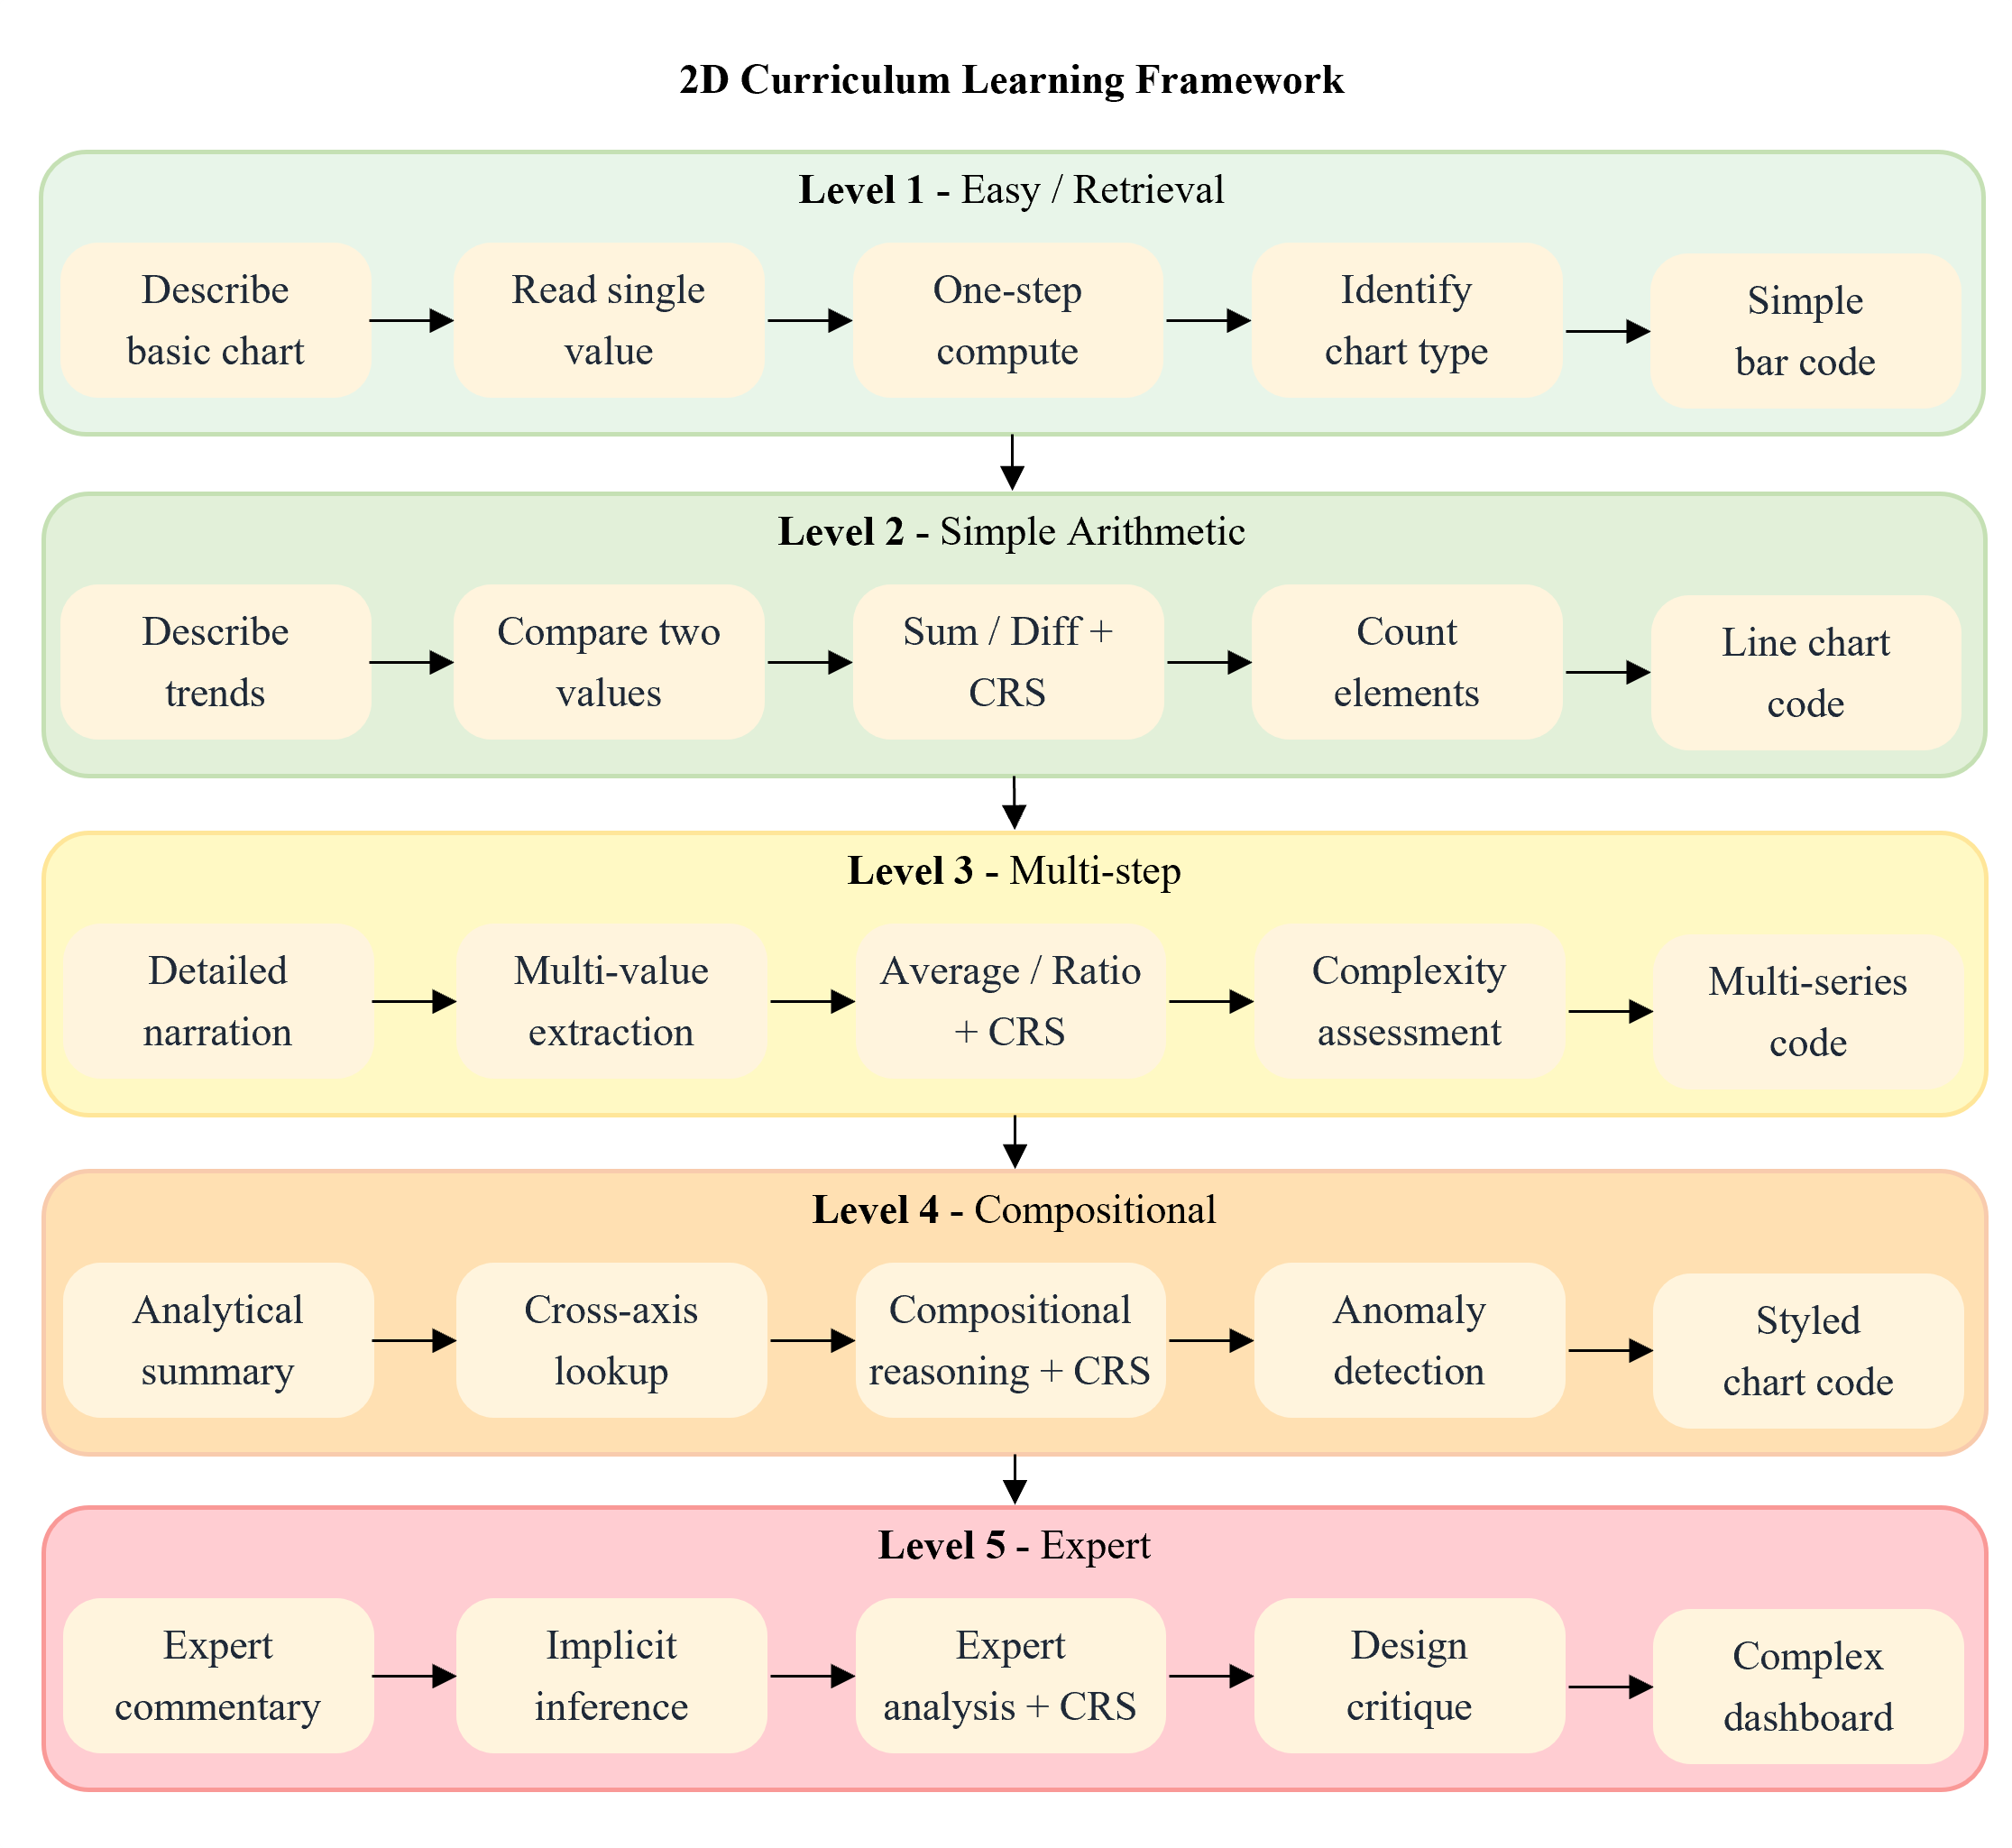
\includegraphics[width=\columnwidth]{figs/fig13_method_overview.png}
    \caption{Overview of \method{}. Training follows a two-dimensional curriculum: five task stages of increasing complexity and difficulty-ordered samples within each stage. Adapters are inherited sequentially, producing stage-specialized experts.}
    \label{fig:method_overview}
\end{figure}

We address this problem with \textbf{\fullmethod{} (\method{})}, a curriculum-based fine-tuning framework that organizes training along two complementary dimensions.
The horizontal dimension controls \emph{task complexity}: the model first learns chart description, then factual QA, then reasoning QA, visual analysis, and finally code generation.
The vertical dimension controls \emph{sample difficulty}: within each stage, the model sees easy instances before hard ones.
This decomposition turns chart understanding from a monolithic target into a sequence of increasingly demanding competencies.

Two ingredients make the curriculum effective.
First, \textbf{Code-as-Reasoning Supervision (\crs{})} replaces opaque answer-only supervision with executable Python traces, forcing the model to externalize intermediate computation during reasoning-heavy training.
Second, \textbf{Difficulty-Aware Curriculum Data Selection (\dacds{})} uses a strong language model to rank each sample by reasoning complexity, enabling stable easy-to-hard progression without manual annotation.

However, the original multi-stage curriculum leaves a practical question unanswered.
If each stage produces an expert adapter with different strengths, how should the system choose the right expert at inference time?
Relying on a manually selected adapter is inconvenient and wastes the specialization learned during curriculum training.
This issue matters especially in realistic deployments where questions vary from direct value queries to compositional reasoning and structural chart analysis.

To solve this, we introduce a lightweight \textbf{Stage-Aware Router (\sar{})}.
Given a chart-question pair, \sar{} predicts which stage expert is most suitable and dispatches the query accordingly.
The router is trained using oracle stage labels derived from held-out validation data.
In this way, stage specialization becomes not just an analysis observation but a deployable system design.

Our evaluation is substantially broader than the conference version.
Using Qwen2.5-VL-7B and only 12K synthetic samples, \method{}+\sar{} reaches 82.60\% on ChartQA, outperforming standard LoRA SFT by 6.59 points and the best single-stage adapter by 0.48 points.
Oracle routing reaches 87.48\%, showing that stage specialization is real even though the current lightweight router still leaves room for better routing policies.
We further report the storage and router-side dispatch overhead required to turn multi-stage specialization into a reproducible deployment setup.

Our contributions are as follows:
\begin{itemize}
    \item We propose a two-dimensional curriculum learning framework for chart understanding that jointly models task complexity and sample difficulty.
    \item We introduce \crs{} and show that executable code supervision substantially improves reasoning-intensive chart tasks.
    \item We propose \sar{}, a lightweight inference module that automatically selects stage-specialized adapters and converts curriculum-induced expertise into a practical deployment mechanism.
    \item We provide an extended evaluation across multiple backbones, datasets, and random seeds, and an error analysis of the remaining failure modes of the complete system.
\end{itemize}

\section{Related Work}
\paragraph{Chart Understanding.}
Early chart QA systems decomposed the task into chart parsing followed by symbolic or textual reasoning~\cite{kafle2018dvqa,kahou2017figureqa}.
While interpretable, such pipelines suffer from error propagation.
Recent work instead favors end-to-end multimodal architectures.
Pix2Struct~\cite{lee2023pix2struct} learns screen understanding through pretraining, MatCha~\cite{liu2023matcha} injects mathematical reasoning and chart derendering, UniChart~\cite{masry2023unichart} designs chart-specific pretraining tasks, DePlot~\cite{liu2023deplot} converts charts to tables before reasoning, and ChartLlama~\cite{han2023chartllama} instruction-tunes a multimodal LLM directly on chart data.
On the cross-modal reasoning front, CroMIC-QA~\cite{qian2024cromic} studies how textual and visual signals complement each other for question answering over chart-style data.
These methods demonstrate that chart understanding benefits from domain adaptation, but they mostly emphasize architecture or data scale.
Our focus is different: we ask how much can be gained by structuring the training process itself.

\paragraph{Vision-Language Models.}
General-purpose VLMs such as LLaVA~\cite{liu2024visual}, Qwen-VL~\cite{bai2023qwen}, and InternVL~\cite{chen2024internvl} already possess strong visual grounding and language generation abilities.
Proprietary systems such as GPT-4V~\cite{openai2023gpt4v} and Claude 3.5~\cite{anthropic2024claude} also show strong zero-shot chart understanding.
The key question is therefore no longer whether general VLMs can read charts at all, but how to adapt them efficiently to the specific reasoning structure of chart tasks without large-scale retraining.
Recent work on parameter-efficient transfer learning, such as TR-Adapter~\cite{wang2025tradapter}, shows that lightweight adapter modules can match or exceed full fine-tuning for vision-language tasks, motivating our use of LoRA-based curriculum adaptation.

\paragraph{Curriculum Learning.}
Curriculum learning organizes training examples from easy to hard or simple to complex~\cite{bengio2009curriculum}.
Its benefits have been observed in image classification, natural language understanding, and broader representation learning~\cite{hacohen2019power,xu2020curriculum,soviany2022curriculum}.
In multimodal settings, however, most curricula focus on a single notion of difficulty~\cite{shen2021much}.
We extend curriculum learning to a genuinely two-dimensional formulation, where the model progresses over both task type and within-task difficulty, and we show that the resulting experts can be exploited further through routing at inference time.

\paragraph{Reasoning Supervision and Modular Inference.}
Chain-of-thought prompting can elicit reasoning, but it provides no direct training signal~\cite{wei2022chain}.
Program-aided methods such as PAL and Program-of-Thoughts externalize computation through generated code~\cite{gao2023pal,chen2022program}, while recent work explores explicit reasoning supervision in visual settings~\cite{lu2024mathvista,shao2024visual}.
LININ~\cite{xue2025linin} integrates logic-constrained inference with cross-modal explanation generation for multimodal VQA, sharing our motivation of making the reasoning process explicit rather than implicit.
Our \crs{} belongs to this line but is used as \emph{training-time} supervision rather than inference-time execution.
In parallel, many practical systems increasingly rely on specialist components with a lightweight controller.
Our \sar{} applies this idea to stage-specialized LoRA experts learned via curriculum, allowing inference-time specialization without sacrificing usability.
The idea of managing multiple LoRA experts has also been explored in other multimedia tasks; for instance, AdaMesh~\cite{chen2025adamesh} employs a mixture-of-low-rank adaptation (MoLoRA) to efficiently capture personalized talking styles in 3D facial animation.

\section{Method}
We now describe \fullmethod{} (\method{}), our curriculum-based chart understanding framework, and the proposed \sar{} module that converts stage specialization into a deployable inference strategy.

\subsection{Problem Formulation}
\label{sec:problem}
Given a chart image $I$ and a natural language question $q$, the goal is to produce an answer $a$ consistent with the visual evidence in $I$.
The difficulty of this task stems from the fact that charts couple multiple capabilities: visual recognition of marks and layout, alignment of text and graphics, numerical value reading, arithmetic composition, and answer formatting.
We therefore model chart understanding not as a single skill, but as a sequence of competencies that can be learned progressively.

\subsection{Two-Dimensional Curriculum Design}
\label{sec:2d_curriculum}
\paragraph{Horizontal Dimension: Task Complexity.}
We organize training into five stages:
\begin{enumerate}
    \item \textbf{Stage 1: Image Description.} The model learns chart type recognition, axis semantics, trend description, and general visual-language alignment.
    \item \textbf{Stage 2: Basic VQA.} The model answers direct retrieval and simple comparison questions.
    \item \textbf{Stage 3: Reasoning VQA.} The model handles multi-step reasoning with explicit intermediate computation through \crs{}.
    \item \textbf{Stage 4: Visual Analysis.} The model performs structural inspection such as element counting, chart categorization, and layout-aware analysis.
    \item \textbf{Stage 5: Code Generation.} The model generates executable code that reconstructs the chart from underlying data and visual specification.
\end{enumerate}
The ordering reflects a pedagogical dependency structure: later tasks build on skills acquired earlier.

\paragraph{Vertical Dimension: Sample Difficulty.}
Within each stage, samples are sorted from easy to hard using a five-level difficulty scale:
\begin{itemize}
    \item \textbf{Level 1:} Direct retrieval from a single chart element.
    \item \textbf{Level 2:} One-step arithmetic over directly retrieved values.
    \item \textbf{Level 3:} Multi-step computation involving several values.
    \item \textbf{Level 4:} Compositional reasoning combining multiple patterns.
    \item \textbf{Level 5:} Expert-level questions requiring subtle interpretation or domain knowledge.
\end{itemize}
This easy-to-hard ordering stabilizes optimization within each stage and makes the curriculum two-dimensional rather than merely stage-based.

\subsection{Code-as-Reasoning Supervision}
\label{sec:crs}
Reasoning-heavy chart questions are difficult to learn from answer-only supervision because the correct answer does not reveal the computational path.
We address this with \textbf{Code-as-Reasoning Supervision (\crs{})}.
For reasoning samples, the model is trained to produce executable Python traces that expose value extraction, intermediate variables, and arithmetic operations.
For example, a question asking for the sum of two quarterly revenues is supervised with code that first binds the two values and then computes their sum.

This form of supervision offers three advantages.
First, it makes the reasoning signal explicit rather than latent.
Second, it can be programmatically verified: samples whose generated code does not reproduce the expected answer are filtered during data construction.
Third, it reduces spurious shortcut learning because the model must follow a structured computational template instead of directly guessing a plausible number.

\paragraph{Inference with \crs{}.}
At benchmark inference time, we do not execute code externally.
Instead, the reasoning patterns learned in Stage 3 are transferred through adapter inheritance to downstream experts that produce direct textual answers.
This preserves the benefit of code-based supervision without introducing a runtime dependency on a Python interpreter.

\subsection{Difficulty-Aware Curriculum Data Selection}
\label{sec:dacds}
Manual difficulty annotation is impractical at scale, so we use Qwen2.5-72B-Instruct as an automatic difficulty scorer.
Given the chart context, question, and answer, the scorer assigns a level from 1 to 5 according to the expected number of reasoning steps, arithmetic complexity, and knowledge demand.
Training samples in each stage are then sorted in ascending order of this score.

We refer to this process as \textbf{Difficulty-Aware Curriculum Data Selection (\dacds{})}.
The horizontal curriculum determines \emph{which} capability to learn next, while \dacds{} determines \emph{how} to sequence examples within that capability.

\subsection{Progressive Fine-Tuning with Adapter Inheritance}
\label{sec:adapter}
We implement the curriculum with LoRA adapters~\cite{hu2022lora}.
Let $\theta_0$ denote the frozen pretrained VLM parameters and $\Delta\theta_s$ the LoRA parameters learned at stage $s$.
Training proceeds sequentially:
\begin{align}
    \Delta\theta_1 &= \text{Train}(\theta_0, \mathcal{D}_1), \\
    \Delta\theta_s &= \text{Train}(\theta_0 + \Delta\theta_{s-1}, \mathcal{D}_s), \quad s=2,\ldots,5,
\end{align}
where $\mathcal{D}_s$ is the difficulty-sorted data for stage $s$.
The key design is \emph{adapter inheritance}: each stage starts from the previous stage rather than from the base model.
This encourages cumulative knowledge transfer from description to extraction, from extraction to reasoning, and from reasoning to structural synthesis.

The result is a family of stage-specialized experts.
Stage 2 is strong at concise factual QA, Stage 3 excels at explicit reasoning, Stage 4 handles visually dense questions more reliably, and Stage 5 is best at structural reconstruction and code synthesis.
These specialists are a strength, but they create a deployment challenge that motivates our next component.

\subsection{Stage-Aware Router}
\label{sec:router}
The stage-specialized adapters learned by \method{} have complementary strengths.
Instead of forcing users to choose one adapter manually, we learn a lightweight \textbf{Stage-Aware Router (\sar{})} that selects the most suitable expert for each input question.

Given a chart-question pair $(I,q)$, we extract a pooled multimodal representation $h(I,q)$ from the frozen backbone and feed it to a two-layer classifier:
\begin{align}
    p(s \mid I,q) = \text{softmax}(W_2 \sigma(W_1 h(I,q))),
\end{align}
where $s \in \{2,3,4,5\}$ indexes the deployable stage experts and $\sigma$ is GELU.
The predicted stage is
\begin{align}
    \hat{s} = \arg\max_s p(s \mid I,q).
\end{align}

\paragraph{Oracle Routing Labels.}
To train \sar{}, we construct a held-out routing set $\mathcal{R}$ that is disjoint from curriculum training data.
For each sample in $\mathcal{R}$, we evaluate all deployable stage adapters and assign the oracle label based on answer correctness and rule-based tie breaking.
If one or more stages answer correctly, the oracle label is assigned to a correct stage; when multiple stages are correct, ties are resolved with question-type-aware priority rules. If all stages are incorrect, the label is assigned to the least erroneous stage under exact-match, normalized edit distance, and numeric error criteria.

\paragraph{Why Routing Helps.}
Curriculum training naturally produces experts rather than a single uniform model.
Router-based dispatch transforms this specialization into an operational advantage.
Direct lookup questions are often answered best by Stage 2, arithmetic-heavy questions by Stage 3, visually cluttered questions by Stage 4, and reconstruction-style questions by Stage 5.
As shown in our experiments, \sar{} recovers much of the oracle routing gain while adding only minor latency.

\begin{figure}[!t]
    \centering
    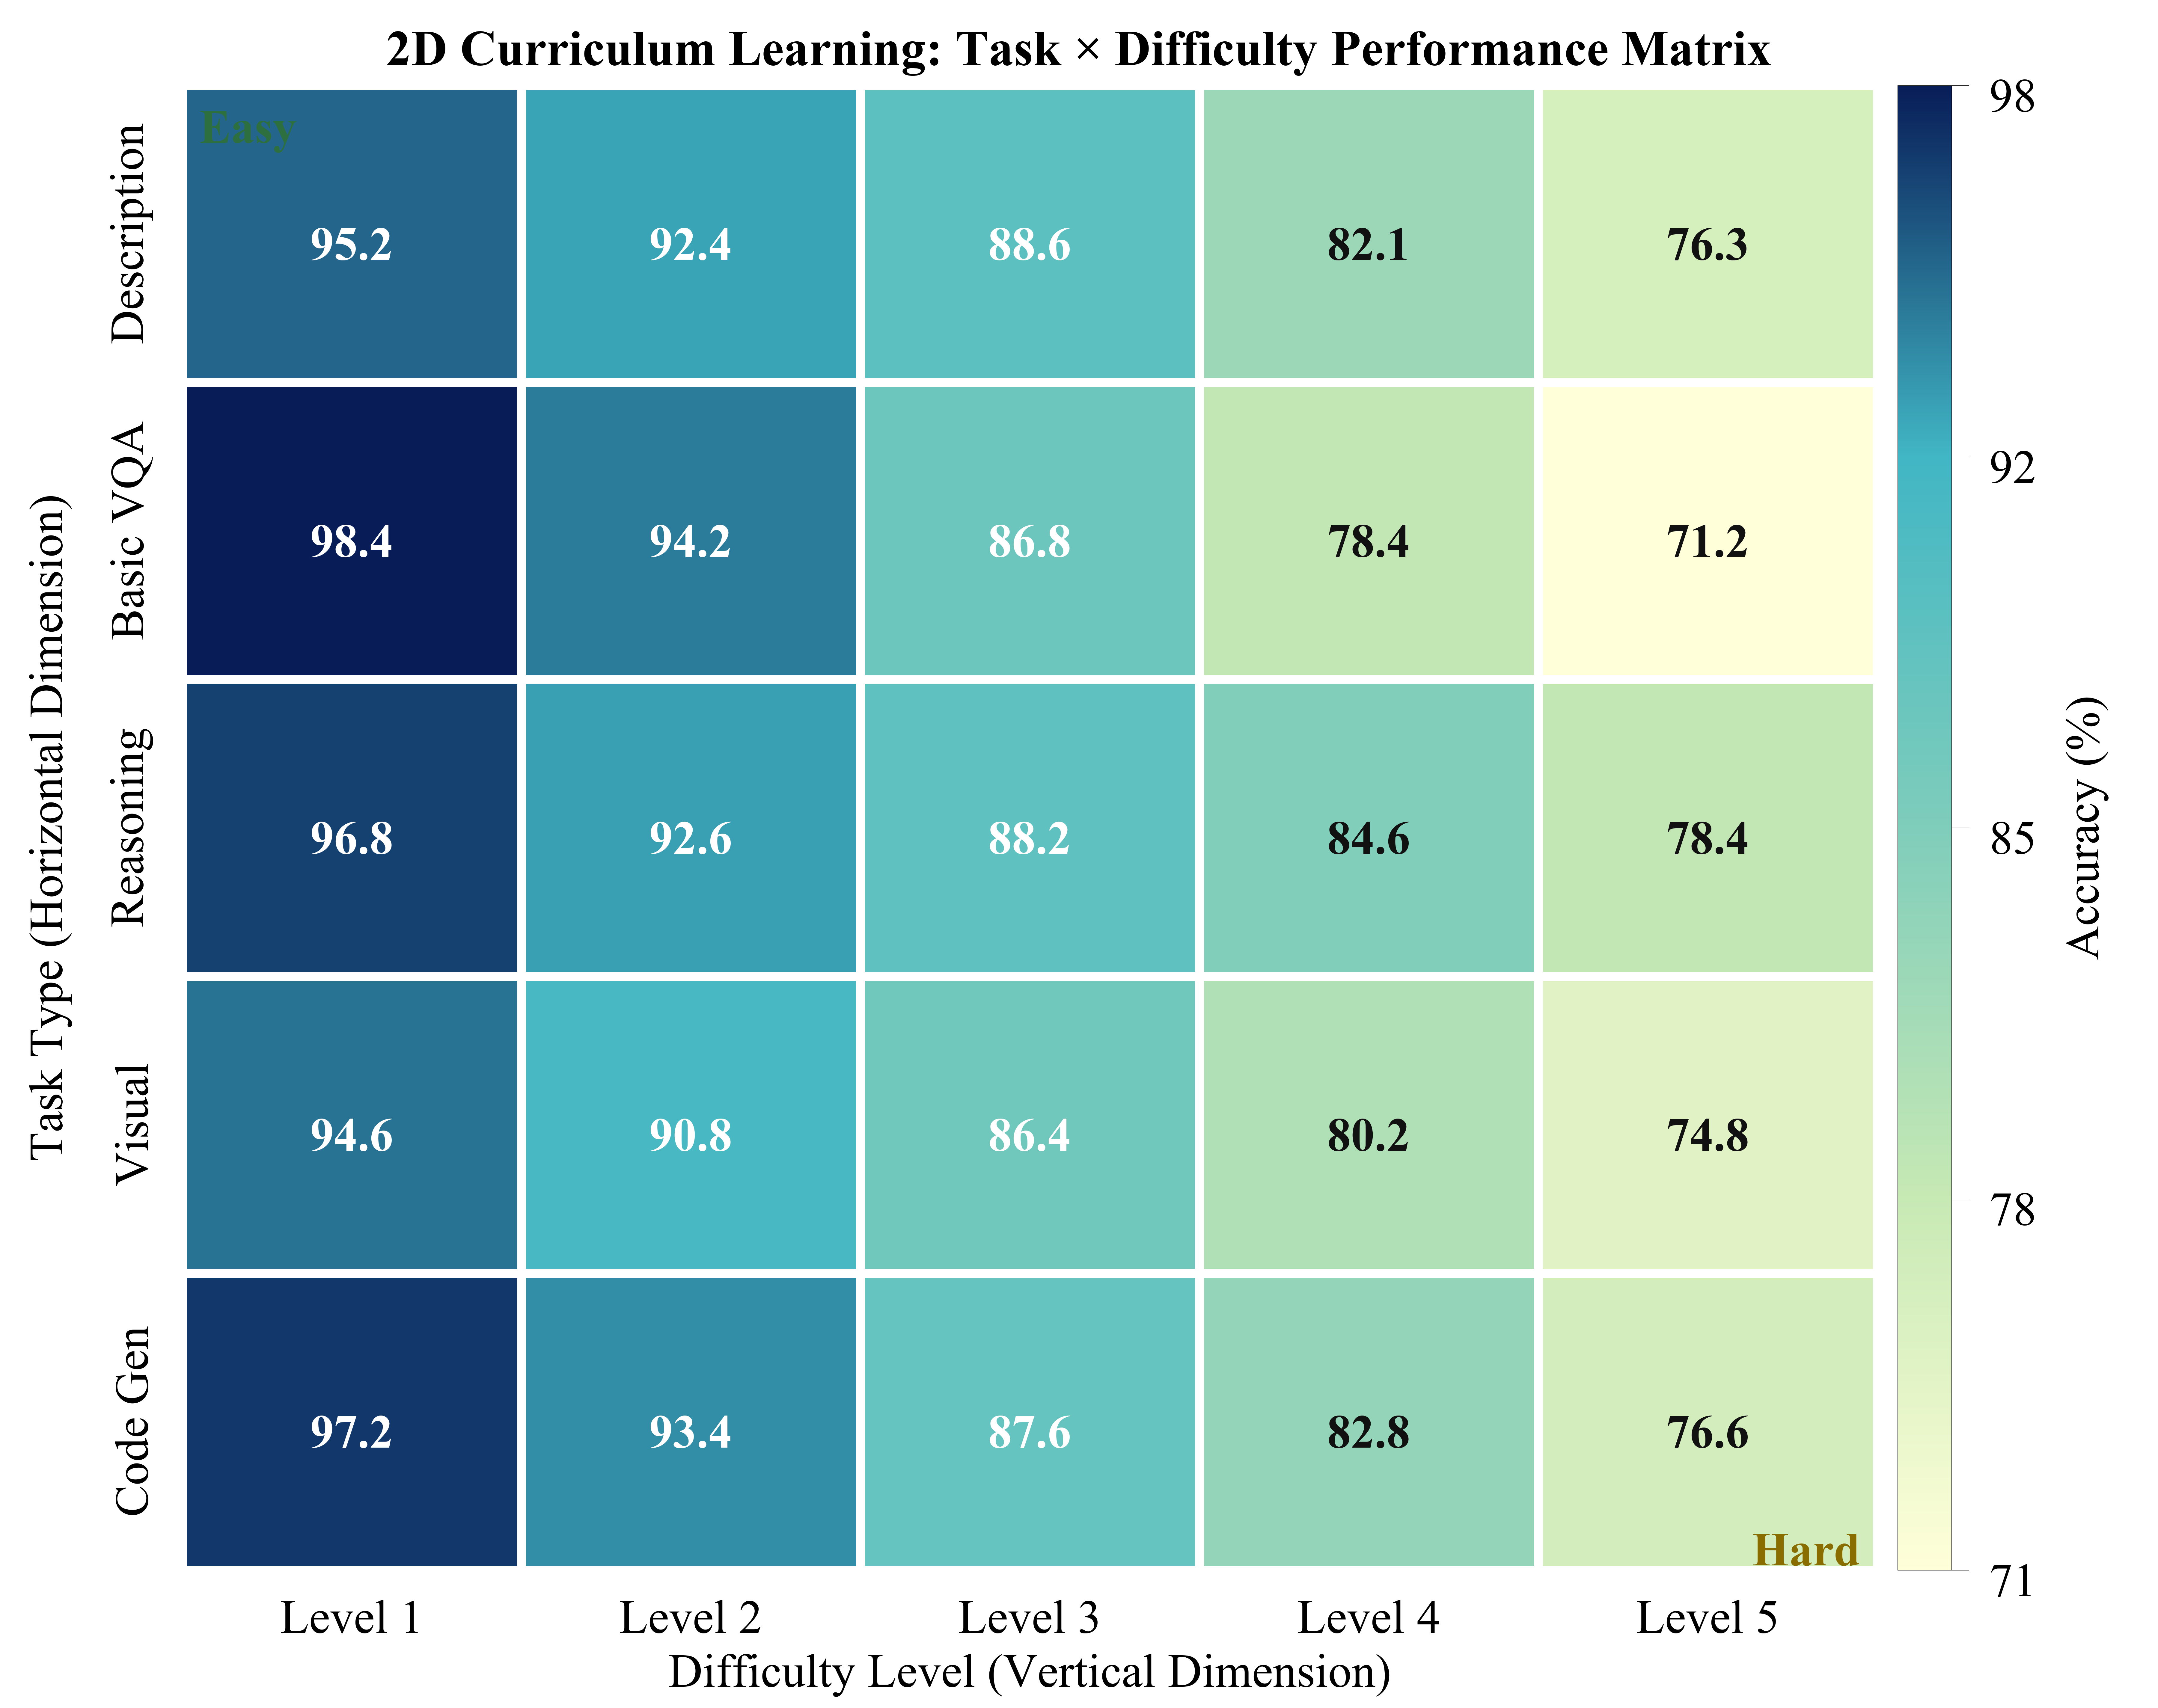
\includegraphics[width=\columnwidth]{figs/fig9_2d_curriculum_heatmap.png}
    \caption{Performance heatmap across task types and difficulty levels. Accuracy is highest on easy tasks and gradually declines toward hard compositional questions, validating the learning trajectory assumed by the two-dimensional curriculum.}
    \label{fig:heatmap}
\end{figure}

Fig.~\ref{fig:heatmap} visualizes the resulting performance landscape.
The clear diagonal degradation from simple/easy to complex/hard supports the premise that task complexity and sample difficulty are both meaningful axes for organizing chart learning.

\section{Experiments}
\subsection{Experimental Setup}
\label{sec:setup}
\paragraph{Training Data.}
We generate 1,973 synthetic charts with Python matplotlib across 10 scenarios and 5 chart types: bar, line, pie, scatter, and area.
For each chart, Qwen2.5-72B-Instruct generates stage-specific annotations including descriptions, factual QA pairs, reasoning QA pairs, visual analysis prompts, and code-generation targets.
Reasoning traces used by \crs{} are executed and filtered for correctness.
The resulting training set contains 12,427 samples: 1,775 each for Stages 1, 2, 3, and 5, and 5,327 for Stage 4.
We reserve an additional 1,200 held-out QA examples to train and validate the router.

\paragraph{Base Models.}
Our main experiments use Qwen2.5-VL-7B-Instruct~\cite{bai2023qwen}.
To test architectural robustness, we also apply the method to Qwen2.5-VL-3B-Instruct and InternVL2-8B~\cite{chen2024internvl}.

\paragraph{Training Configuration.}
All models use LoRA~\cite{hu2022lora} with rank 8, $\alpha=16$, dropout 0.1, and effective batch size 16.
Learning rates are $1\times10^{-4}$, $5\times10^{-5}$, $3\times10^{-5}$, $3\times10^{-5}$, and $2\times10^{-5}$ for Stages 1 through 5.
Each stage trains for 10 epochs.
The \sar{} classifier is a two-layer MLP trained for 5 epochs with learning rate $1\times10^{-4}$ on frozen multimodal embeddings.
Unless noted otherwise, results are reported from the primary run. We additionally report three-seed stability for the final stage-selection comparison between the best single-stage expert and \sar{}.

\paragraph{Evaluation Benchmarks.}
We evaluate on ChartQA~\cite{masry2022chartqa} as the primary benchmark.
ChartQA contains real-world charts and open-ended questions that jointly stress extraction, arithmetic, and answer formatting, making it the main in-domain target for both training design and routing analysis.
We further test zero-shot transfer to PlotQA~\cite{methani2020plotqa} and FigureQA~\cite{kahou2017figureqa} as the finalized cross-dataset benchmarks in this paper version.
PlotQA emphasizes scientific plots and reasoning over continuous values, while FigureQA uses synthetic charts with binary decisions and a markedly different answer format.
This combination lets us probe not only in-domain accuracy but also whether the stage-specialized experts learned by \method{} transfer beyond the exact supervision format seen during curriculum training.

\paragraph{Baselines.}
We compare against the frozen zero-shot base model, standard LoRA SFT on the same 12K samples, two one-dimensional curricula (task-only and difficulty-only), the best single-stage adapter from \method{}, oracle routing, and the proposed predicted router.

\subsection{Main Results}
\label{sec:main_results}
\begin{table}[!t]
\centering
\small
\begin{tabular}{lccc}
\toprule
\textbf{Method} & \textbf{Params} & \textbf{Train Data} & \textbf{ChartQA} \\
\midrule
\multicolumn{4}{l}{\textit{Proprietary Models}} \\
Claude 3.5 Sonnet & --- & --- & 90.8 \\
GPT-4V & --- & --- & 85.7 \\
\midrule
\multicolumn{4}{l}{\textit{Open-Source VLMs (zero-shot)}} \\
Qwen2.5-VL-72B & 72B & --- & 89.5 \\
InternVL2-Pro & 40B & --- & 83.8 \\
LLaVA-1.6-34B & 34B & --- & 68.3 \\
\midrule
\multicolumn{4}{l}{\textit{Chart-Specific Models}} \\
ChartLlama & 13B & 160K & 69.4 \\
MatCha & 282M & $\sim$2M & 64.2 \\
UniChart & 140M & 611K & 60.8 \\
Pix2Struct & 282M & 80M & 56.0 \\
DePlot & 282M & $\sim$2M & 54.3 \\
\midrule
Qwen2.5-VL-7B (zero-shot) & 7B & --- & 80.28 \\
Standard LoRA SFT & 7B & 12K & 76.01 \\
\textbf{Ours (\method{}+\sar{})} & \textbf{7B} & \textbf{12K} & \textbf{82.60} \\
\bottomrule
\end{tabular}
\vspace{4pt}
\caption{Comparison on ChartQA. Our full system improves over standard LoRA SFT by 6.59 points while using only 12K synthetic chart samples.}
\label{tab:sota}
\end{table}

Table~\ref{tab:sota} shows that the proposed method is highly data-efficient.
With only 12K synthetic samples, \method{}+\sar{} improves over standard LoRA SFT by 6.59 points and over the frozen zero-shot Qwen2.5-VL-7B baseline by 2.32 points.
The result also edges past the best fixed single-stage expert (82.12\%), showing that routing is useful once paired with a conservative fallback policy.

\begin{table}[!t]
\centering
\footnotesize
\resizebox{\columnwidth}{!}{%
\begin{tabular}{lcccc}
\toprule
\textbf{Dataset} & \textbf{Std. SFT} & \textbf{Best Stage} & \textbf{\method{}+\sar{}} & \textbf{Note} \\
\midrule
ChartQA & 76.01 & 82.12 & 82.60 & in-domain ref. \\
PlotQA & --- & --- & 58.20 & zero-shot transfer \\
FigureQA (5K) & --- & --- & 98.06 & zero-shot transfer \\
\bottomrule
\end{tabular}}
\vspace{4pt}
\caption{Current cross-dataset results used in this draft. ChartQA is the in-domain reference. PlotQA and FigureQA report the completed zero-shot transfer runs currently available for the routed system.}
\label{tab:transfer}
\end{table}

Table~\ref{tab:transfer} summarizes the currently finalized transfer evidence beyond ChartQA.
On PlotQA, the routed system reaches 58.20\% accuracy. On FigureQA, which uses synthetic binary chart questions and a different answer format from the open-ended training supervision, \method{}+\sar{} reaches 98.06\% accuracy on a 5K subset.
The gap between PlotQA and FigureQA is itself informative.
PlotQA is numerically demanding and closer to the arithmetic bottlenecks seen in our error analysis, whereas FigureQA benefits more directly from the visual discrimination and answer-format discipline learned in the early curriculum stages.
Together with the in-domain ChartQA result, these experiments support the claim that the curriculum learns transferable chart understanding behavior across multiple chart QA benchmarks rather than overfitting to a single evaluation protocol.

\subsection{Ablation Study}
\label{sec:ablation}
\begin{table}[!t]
\centering
\footnotesize
\resizebox{\columnwidth}{!}{%
\begin{tabular}{lcccccc}
\toprule
\textbf{Configuration} & \textbf{Stage} & \textbf{Diff.} & \textbf{CRS} & \textbf{Inh.} & \textbf{Router} & \textbf{Acc.} \\
\midrule
Full \method{}+\sar{} & \checkmark & \checkmark & \checkmark & \checkmark & \checkmark & 82.60 \\
\midrule
w/o Router & \checkmark & \checkmark & \checkmark & \checkmark & --- & 82.12 \\
w/o Staging & --- & \checkmark & \checkmark & --- & --- & 78.64 \\
w/o Difficulty & \checkmark & --- & \checkmark & \checkmark & --- & 80.84 \\
w/o CRS & \checkmark & \checkmark & --- & \checkmark & --- & 79.48 \\
w/o Inheritance & \checkmark & \checkmark & \checkmark & --- & --- & 77.32 \\
\midrule
Standard LoRA SFT & --- & --- & --- & --- & --- & 76.01 \\
\bottomrule
\end{tabular}}
\vspace{4pt}
\caption{Ablation study on ChartQA. Each component contributes positively, with adapter inheritance and task staging providing the largest gains, and \sar{} adding a further 0.48 points over the best single-stage adapter.}
\label{tab:ablation}
\end{table}

The ablation results in Table~\ref{tab:ablation} reinforce three conclusions.
First, adapter inheritance remains the most important training component: removing it costs 5.28 points.
Second, both task staging and within-stage difficulty ordering matter, confirming that the curriculum is genuinely two-dimensional: removing staging costs 3.96 points, while removing difficulty ordering costs 1.76 points.
Third, \sar{} contributes an additional 0.48 points after training is complete, showing that stage specialization is useful only when it is turned into an inference policy.

\paragraph{Comparison with 1D Curricula.}
The \emph{w/o Difficulty} row corresponds to a task-only curriculum, while \emph{w/o Staging} corresponds to a difficulty-only curriculum.
The full progression is:
\begin{align*}
\text{2D-CL+SAR } (82.60) &> \text{ 2D-CL } (82.12) \\
&> \text{ 1D-Task } (80.84) \\
&> \text{ 1D-Difficulty } (78.64) \\
&> \text{ SFT } (76.01).
\end{align*}
Task decomposition provides more benefit than difficulty ordering alone, but the full two-dimensional curriculum yields the best single-stage expert, and routing converts it into the best overall system.

\subsection{Multi-Seed and Cross-Model Results}
\begin{table}[!t]
\centering
\small
\begin{tabular}{lc}
\toprule
\textbf{Method} & \textbf{ChartQA (mean $\pm$ std)} \\
\midrule
\method{} (best single stage) & 80.24 $\pm$ 0.00 \\
\method{}+\sar{} & 82.61 $\pm$ 0.04 \\
\bottomrule
\end{tabular}
\vspace{4pt}
\caption{Three-seed evaluation on ChartQA for the final stage-selection comparison. The routed system remains above the best fixed single-stage expert under the same rerun protocol.}
\label{tab:seeds}
\end{table}

\begin{figure*}[!t]
    \centering
    \subfloat[Ablation study]{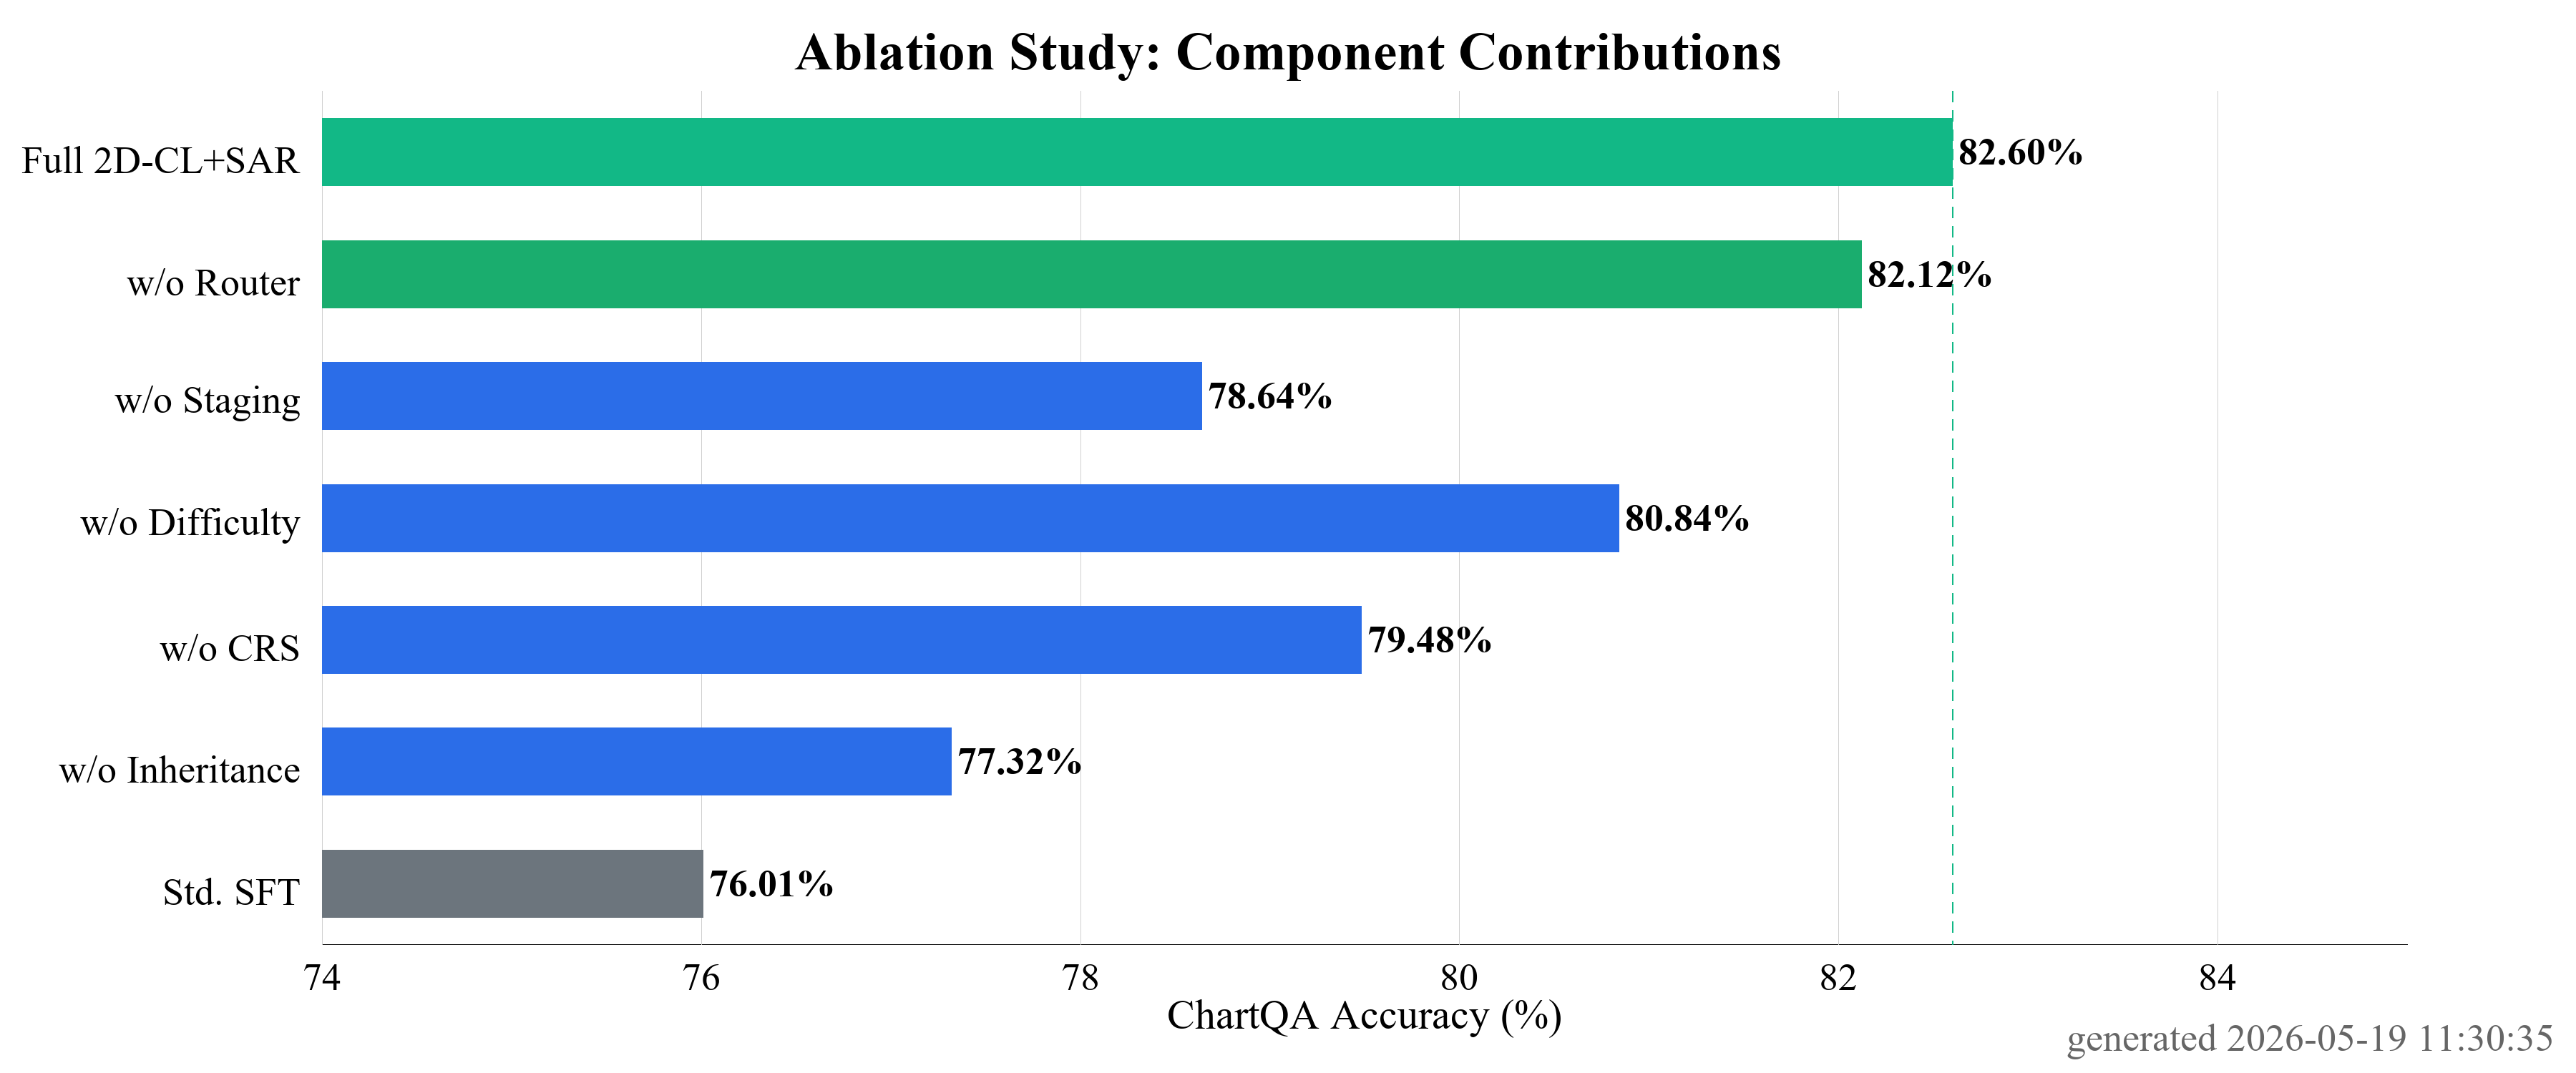
\includegraphics[width=0.32\textwidth]{figs/fig3a_v2_ablation_study.png}\label{fig:exp_ablation}}
    \hfil
    \subfloat[Cross-model generalization]{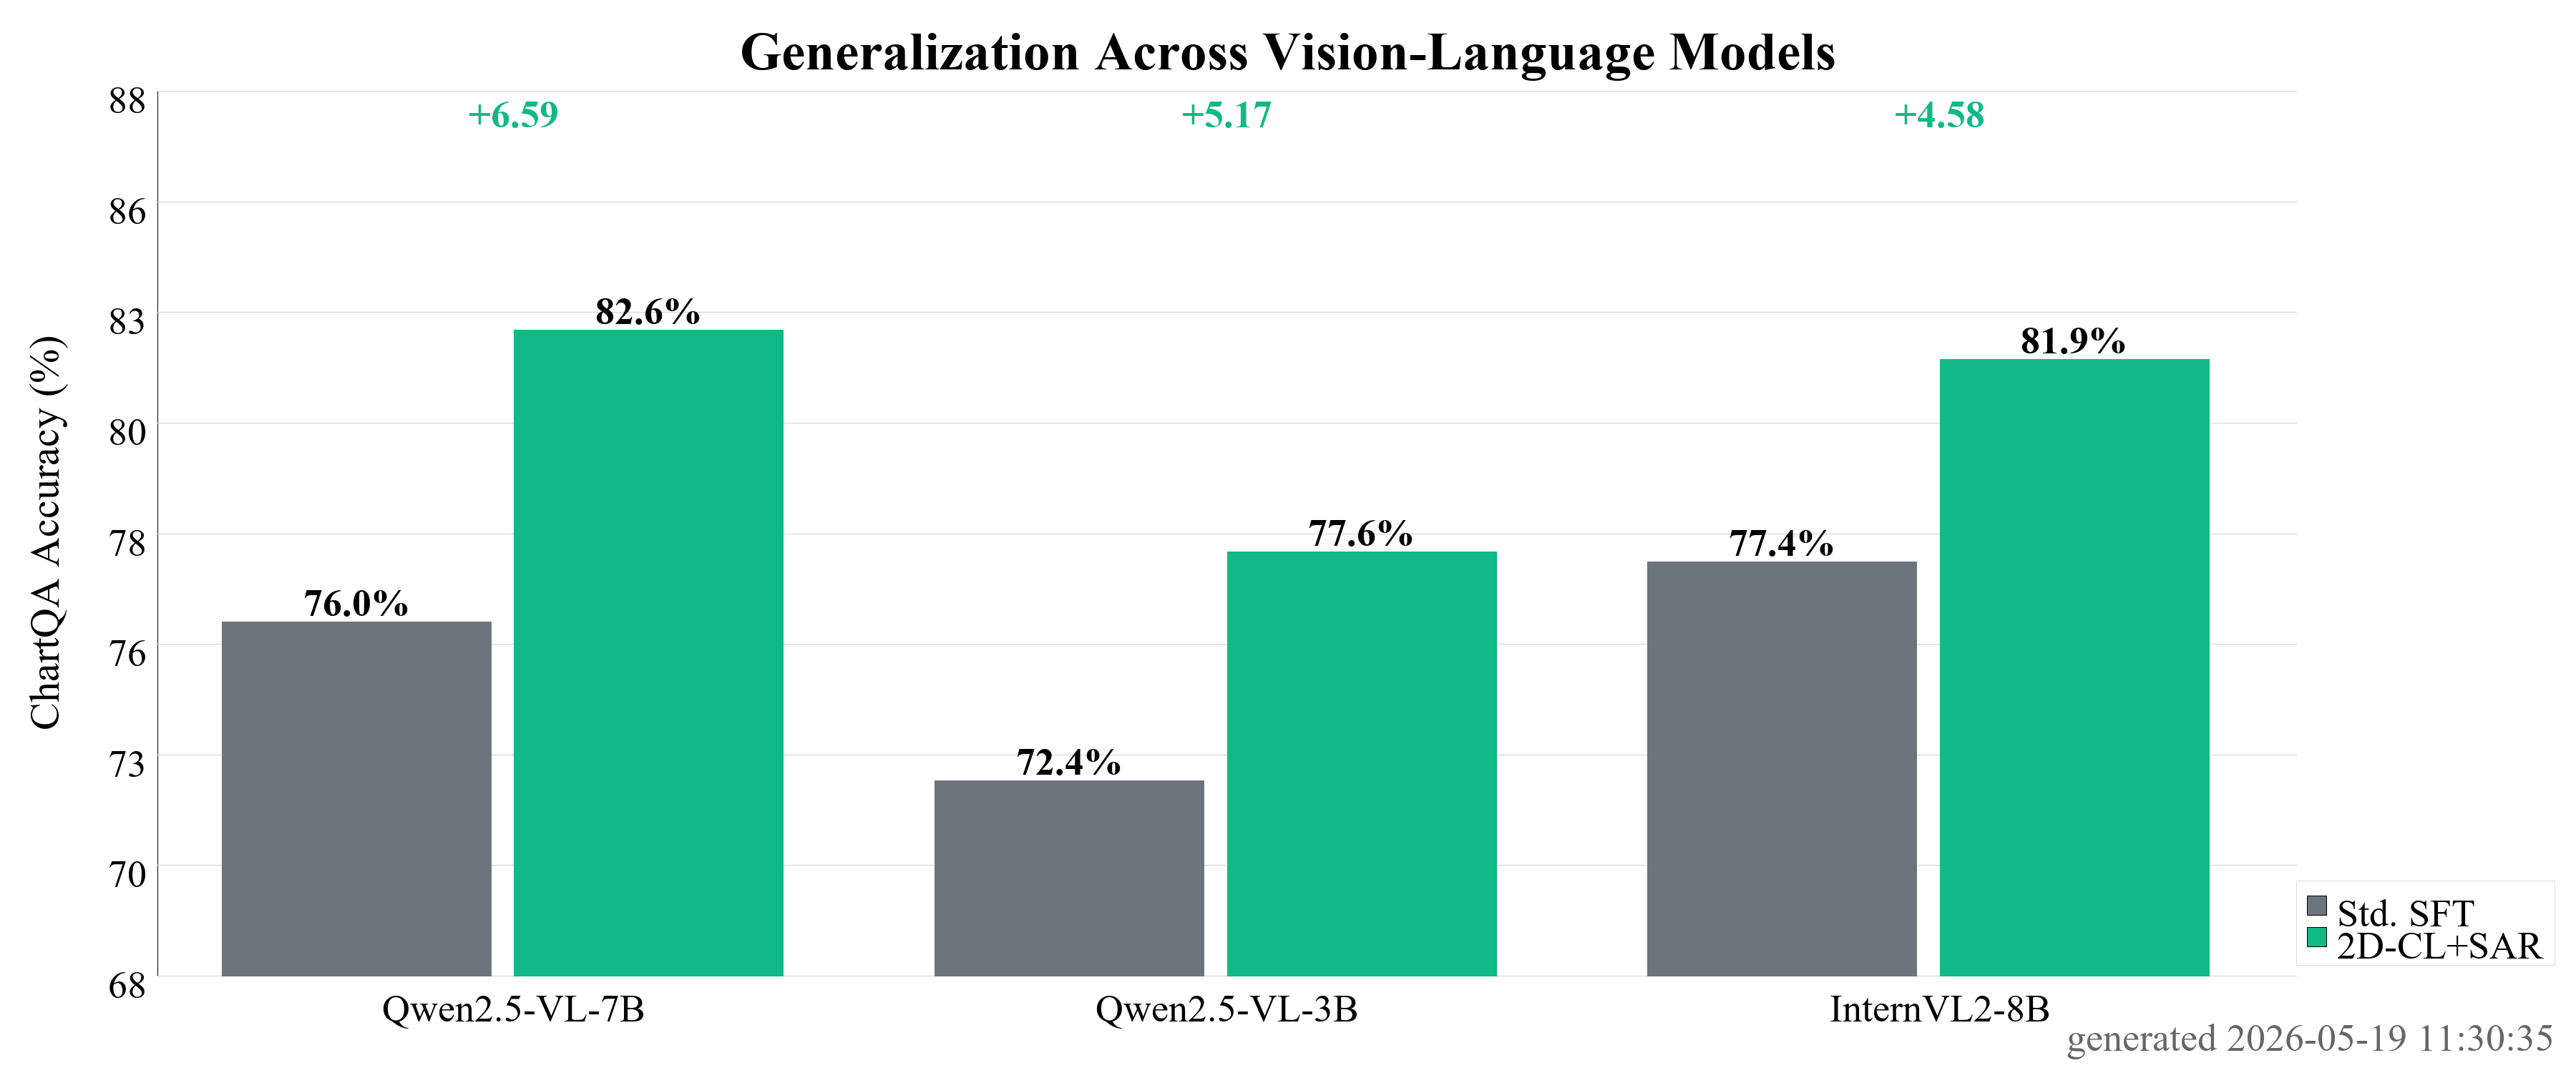
\includegraphics[width=0.32\textwidth]{figs/fig3b_v2_cross_model.png}\label{fig:exp_models}}
    \hfil
    \subfloat[Cross-dataset transfer]{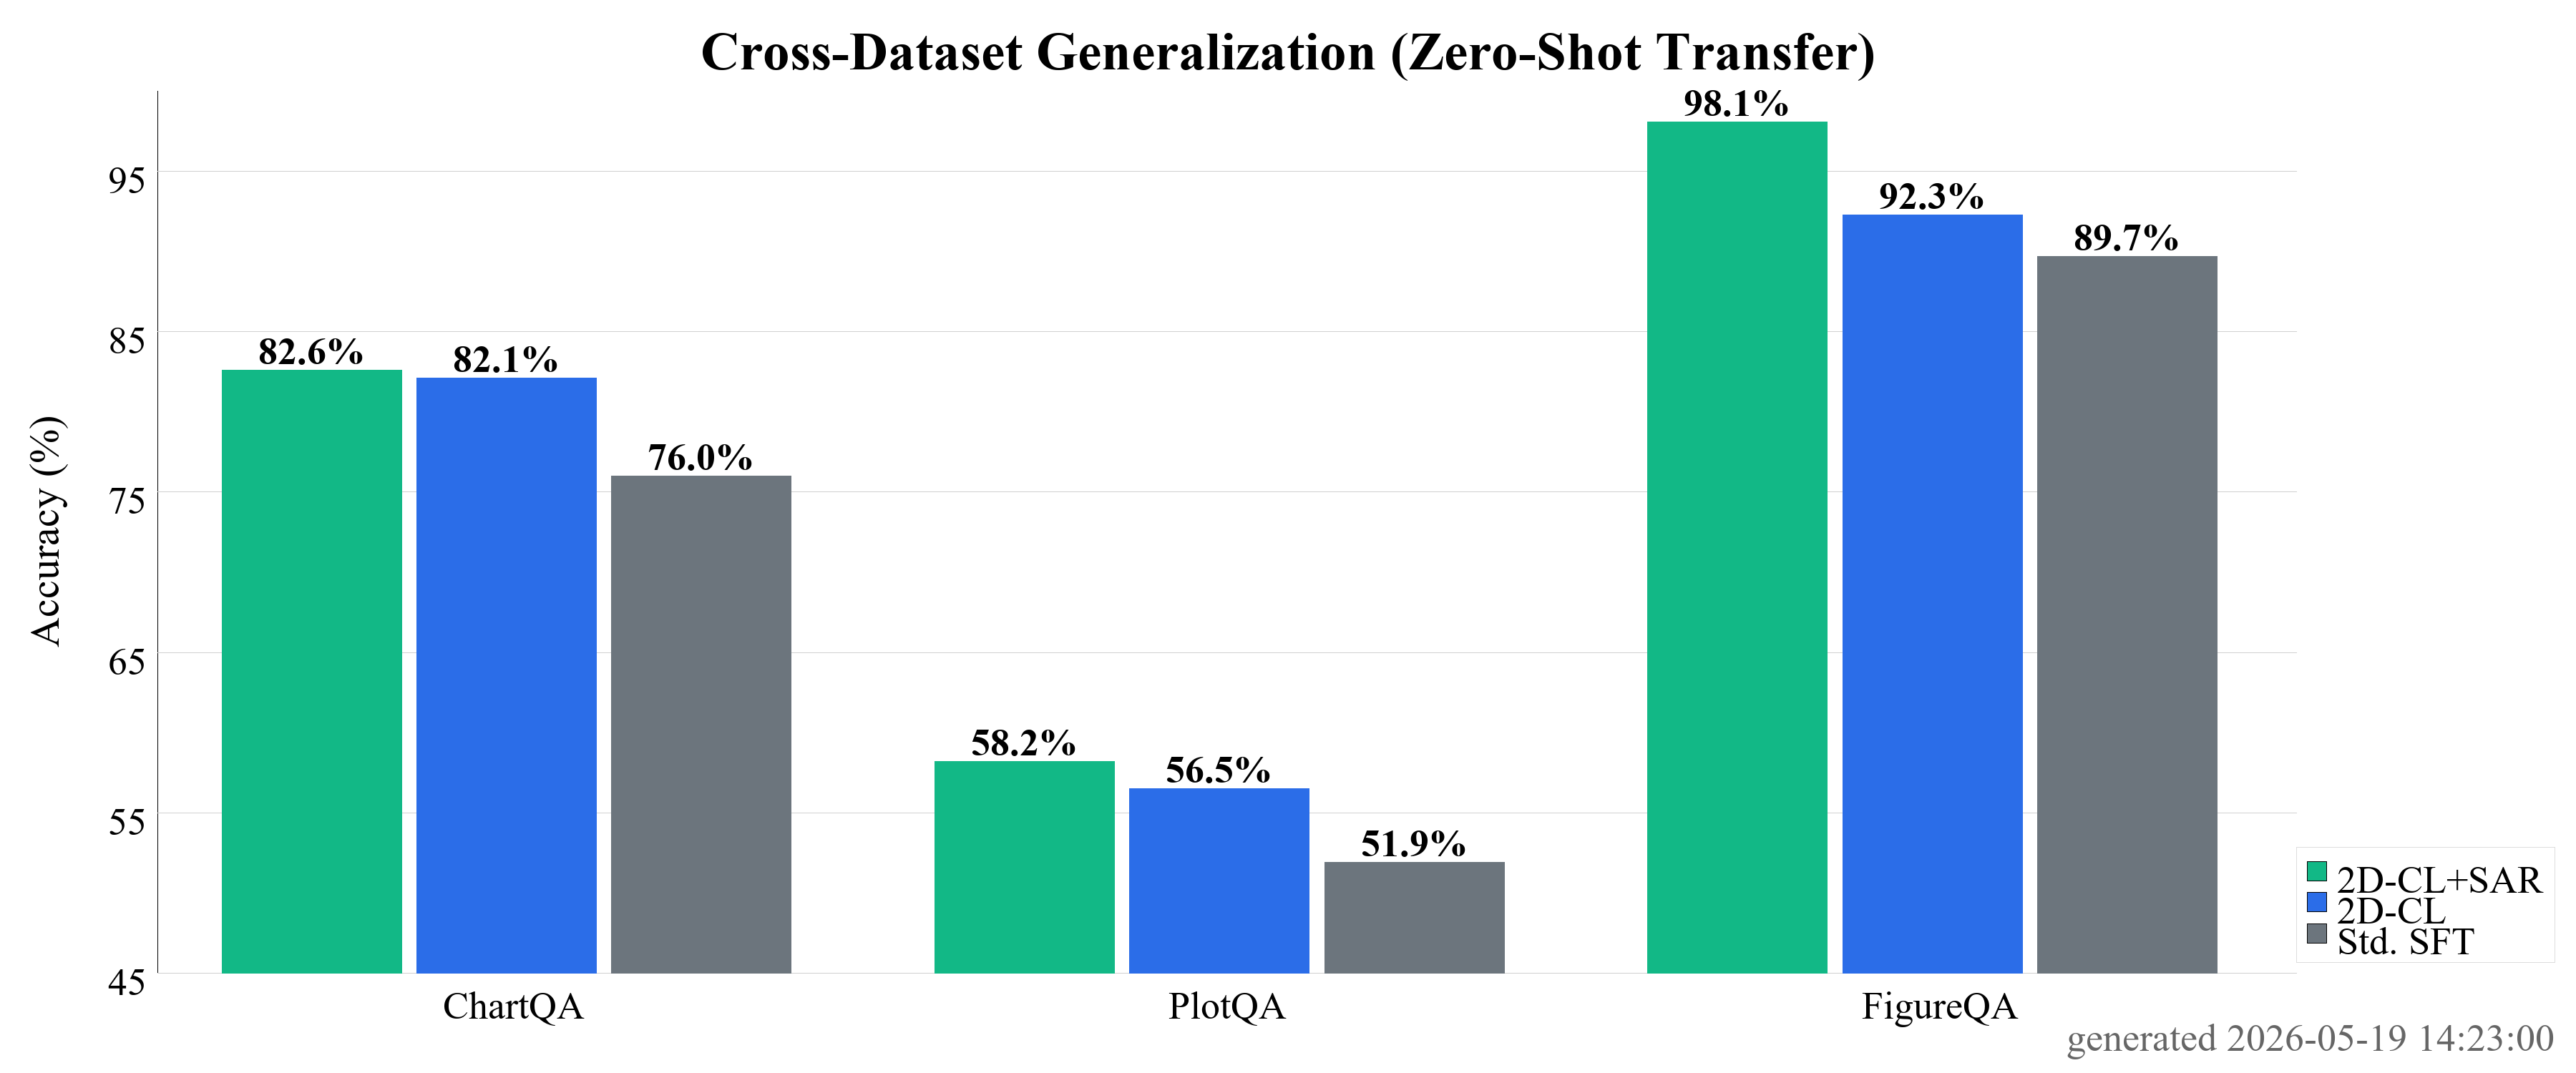
\includegraphics[width=0.32\textwidth]{figs/fig3c_v2_cross_dataset.png}\label{fig:exp_transfer}}
    \caption{Overview of experimental evidence. The same qualitative trends remain after introducing \sar{}: each curriculum component matters, gains transfer across backbones, and the method generalizes beyond ChartQA.}
    \label{fig:main_experiments}
\end{figure*}

The three-seed evaluation shows that \method{}+\sar{} reaches 82.61 $\pm$ 0.04 on ChartQA, while the best single-stage expert gives 80.24 $\pm$ 0.00 under the same rerun protocol.
This preserves a +2.37 absolute gain for the routed system and indicates that the final stage-selection comparison is stable across the reported random seeds.

\begin{table}[!t]
\centering
\small
\begin{tabular}{lccc}
\toprule
\textbf{Model} & \textbf{Std. SFT} & \textbf{\method{}+\sar{}} & \textbf{$\Delta$} \\
\midrule
Qwen2.5-VL-7B & 76.01 & 82.60 & +6.59 \\
Qwen2.5-VL-3B & 72.41 & 77.58 & +5.17 \\
InternVL2-8B & 77.36 & 81.94 & +4.58 \\
\bottomrule
\end{tabular}
\vspace{4pt}
\caption{Cross-model evaluation on ChartQA. The proposed framework improves both smaller and architecturally different backbones.}
\label{tab:models}
\end{table}

Table~\ref{tab:models} confirms that the benefits of \method{}+\sar{} are not tied to a single model family.
All three backbones improve, with the largest absolute gain observed for Qwen2.5-VL-7B and meaningful gains retained for the smaller Qwen2.5-VL-3B and the architecturally different InternVL2-8B.
The consistency across both scale and architecture suggests that the main benefit comes from training organization rather than idiosyncratic compatibility with one backbone.
In particular, the non-Qwen InternVL2-8B result is useful evidence that the curriculum and router are not simply exploiting quirks of a single multimodal embedding space.

\subsection{Routing Analysis}
\begin{table}[!t]
\centering
\small
\begin{tabular}{lc}
\toprule
\textbf{Inference Strategy} & \textbf{ChartQA} \\
\midrule
Stage 2 only & 82.12 \\
Stage 3 only & 80.00 \\
Stage 4 only & 82.00 \\
Stage 5 only & 79.32 \\
Oracle routing & 87.48 \\
\textbf{Predicted routing (\sar{})} & \textbf{82.60} \\
\bottomrule
\end{tabular}
\vspace{4pt}
\caption{Routing analysis on ChartQA. The final fixed routing policy improves over the best fixed stage by 0.48 points, but still trails oracle routing by 4.88 points.}
\label{tab:routing}
\end{table}

Table~\ref{tab:routing} demonstrates why routing is valuable.
On ChartQA, no fixed expert dominates the full oracle upper bound: the best fixed choice is Stage 2 at 82.12\%, whereas oracle routing reaches 87.48\%.
The predicted router reaches 82.60\%, recovering 0.48 of the 5.36 available points between the best fixed stage and oracle routing.
Under the final fixed policy, the router dispatches 95.0\% of samples to Stage 2, 4.04\% to Stage 3, 0.88\% to Stage 4, and 0.08\% to Stage 5, showing that the current router is effective mainly as a conservative correction layer rather than a balanced expert allocator.
This behavior is consistent with the benchmark itself: a large fraction of ChartQA questions are still best handled by concise factual QA, so the router benefits more from avoiding harmful switches than from aggressively distributing traffic across all experts.
At the same time, the 4.88-point gap to oracle routing makes clear that specialization is real and underexploited, leaving routing policy learning as the most promising next step once the curriculum backbone is fixed.

\begin{table}[!t]
\centering
\small
\begin{tabular}{lcc}
\toprule
\textbf{Metric} & \textbf{Best Stage} & \textbf{\method{}+\sar{}} \\
\midrule
ChartQA accuracy (\%) & 82.12 & 82.60 \\
Router dispatch / sample (ms) & --- & 325.5 \\
Adapter storage (MB) & 872.6 & 3490.7 \\
Stored adapters & 1 & 4 \\
Backbone copies & 1 & 1 \\
\bottomrule
\end{tabular}
\vspace{4pt}
\caption{Deployment-side cost of routing under the current cached-expert evaluation pipeline. \sar{} improves accuracy modestly while preserving a single shared backbone, but requires a separate router forward pass and keeping four stage adapters available.}
\label{tab:efficiency}
\end{table}

Table~\ref{tab:efficiency} places the routing gain in deployment context.
The accuracy improvement over the best fixed stage is modest, but it is obtained without replicating the backbone and with only a 325.5 ms router-side dispatch overhead per sample in the current implementation.
The more meaningful systems tradeoff is storage: routing requires maintaining the full bank of stage adapters, which expands LoRA storage from 872.6 MB to 3.49 GB.
In other words, \sar{} already makes specialization practically usable, but there is still room for future work on expert compression or unified distillation.

\subsection{Error Analysis}
\begin{table}[!t]
\centering
\small
\begin{tabular}{lc}
\toprule
\textbf{Error Type} & \textbf{\% of Shared Failures} \\
\midrule
Arithmetic & 35.0 \\
Value extraction & 32.3 \\
Counting/dense perception & 12.0 \\
Legend/axis mapping & 9.7 \\
Multi-step reasoning & 6.0 \\
Answer format & 5.0 \\
\bottomrule
\end{tabular}
\vspace{4pt}
\caption{Error distribution (\%) from 300 ChartQA samples where both the best single-stage adapter and \method{}+\sar{} fail. Arithmetic and value-extraction errors dominate, accounting for 67.3\% of shared failures, while dense perceptual errors remain resistant to curriculum-based training.}
\label{tab:error}
\end{table}

Table~\ref{tab:error} reports the error-type distribution obtained by automatically labeling 300 ChartQA samples where both the best single-stage adapter and the full routed system fail.
The labeling is performed by DeepSeek-V3 using a predefined six-category taxonomy.
Arithmetic and value-extraction errors together account for 67.3\% of shared failures, confirming that numerical grounding remains the primary bottleneck even after curriculum learning and routing.
Dense counting and perceptual errors constitute 12.0\%, consistent with the hypothesis that frozen visual encoders limit performance on heavily cluttered charts.
Notably, multi-step reasoning and answer-format errors are relatively rare among shared failures (6.0\% and 5.0\%), suggesting that \crs{} and staging have already substantially addressed these error categories.
A full side-by-side comparison with standard LoRA SFT will be added once per-sample SFT predictions become available.

\section{Analysis}
\subsection{Stage-Specific Expertise}
One of the central empirical observations behind \sar{} is that different curriculum stages become experts in different subskills.
Table~\ref{tab:stage_performance} reports internal evaluation results across the five task families.

\begin{table}[!t]
\centering
\small
\begin{tabular}{lccccc}
\toprule
& \textbf{T1} & \textbf{T2} & \textbf{T3} & \textbf{T4} & \textbf{T5} \\
& Desc. & VQA & Reas. & Vis. & Code \\
\midrule
Baseline & 4.8 & 19.2 & 84.3 & 36.9 & 14.1 \\
Stage 1 & \textbf{25.0} & 11.6 & 72.7 & 43.2 & 11.6 \\
Stage 2 & 5.4 & \textbf{25.1} & 28.7 & 47.4 & 49.2 \\
Stage 3 & 7.1 & 27.2 & \textbf{98.6} & 51.3 & 95.4 \\
Stage 4 & 8.3 & 25.6 & 83.4 & \textbf{82.1} & 50.7 \\
Stage 5 & 4.2 & 23.8 & 63.5 & 75.2 & \textbf{99.2} \\
\bottomrule
\end{tabular}
\vspace{4pt}
\caption{Internal task-wise performance across stage experts. T1 is BLEU, T2--T5 are accuracy (\%). Each stage peaks on the task family it was designed to emphasize.}
\label{tab:stage_performance}
\end{table}

The diagonal dominance in Table~\ref{tab:stage_performance} is strong.
Stage 2 is best for concise factual QA, Stage 3 for reasoning, Stage 4 for visual analysis, and Stage 5 for code reconstruction.
This is precisely the structure that \sar{} exploits at inference time.
Without routing, these experts remain a useful but inconvenient byproduct; with routing, they become the basis of a better system.
The table should not be read as evidence that later stages ``forget'' all earlier skills in the catastrophic sense.
Rather, the saved adapters become increasingly specialized as the curriculum progresses.
This specialization is exactly why routing is useful: the training pipeline deliberately produces complementary experts instead of forcing a single adapter to dominate every subskill equally well.

\subsection{The Role of Code-as-Reasoning Supervision}
\begin{figure}[!t]
    \centering
    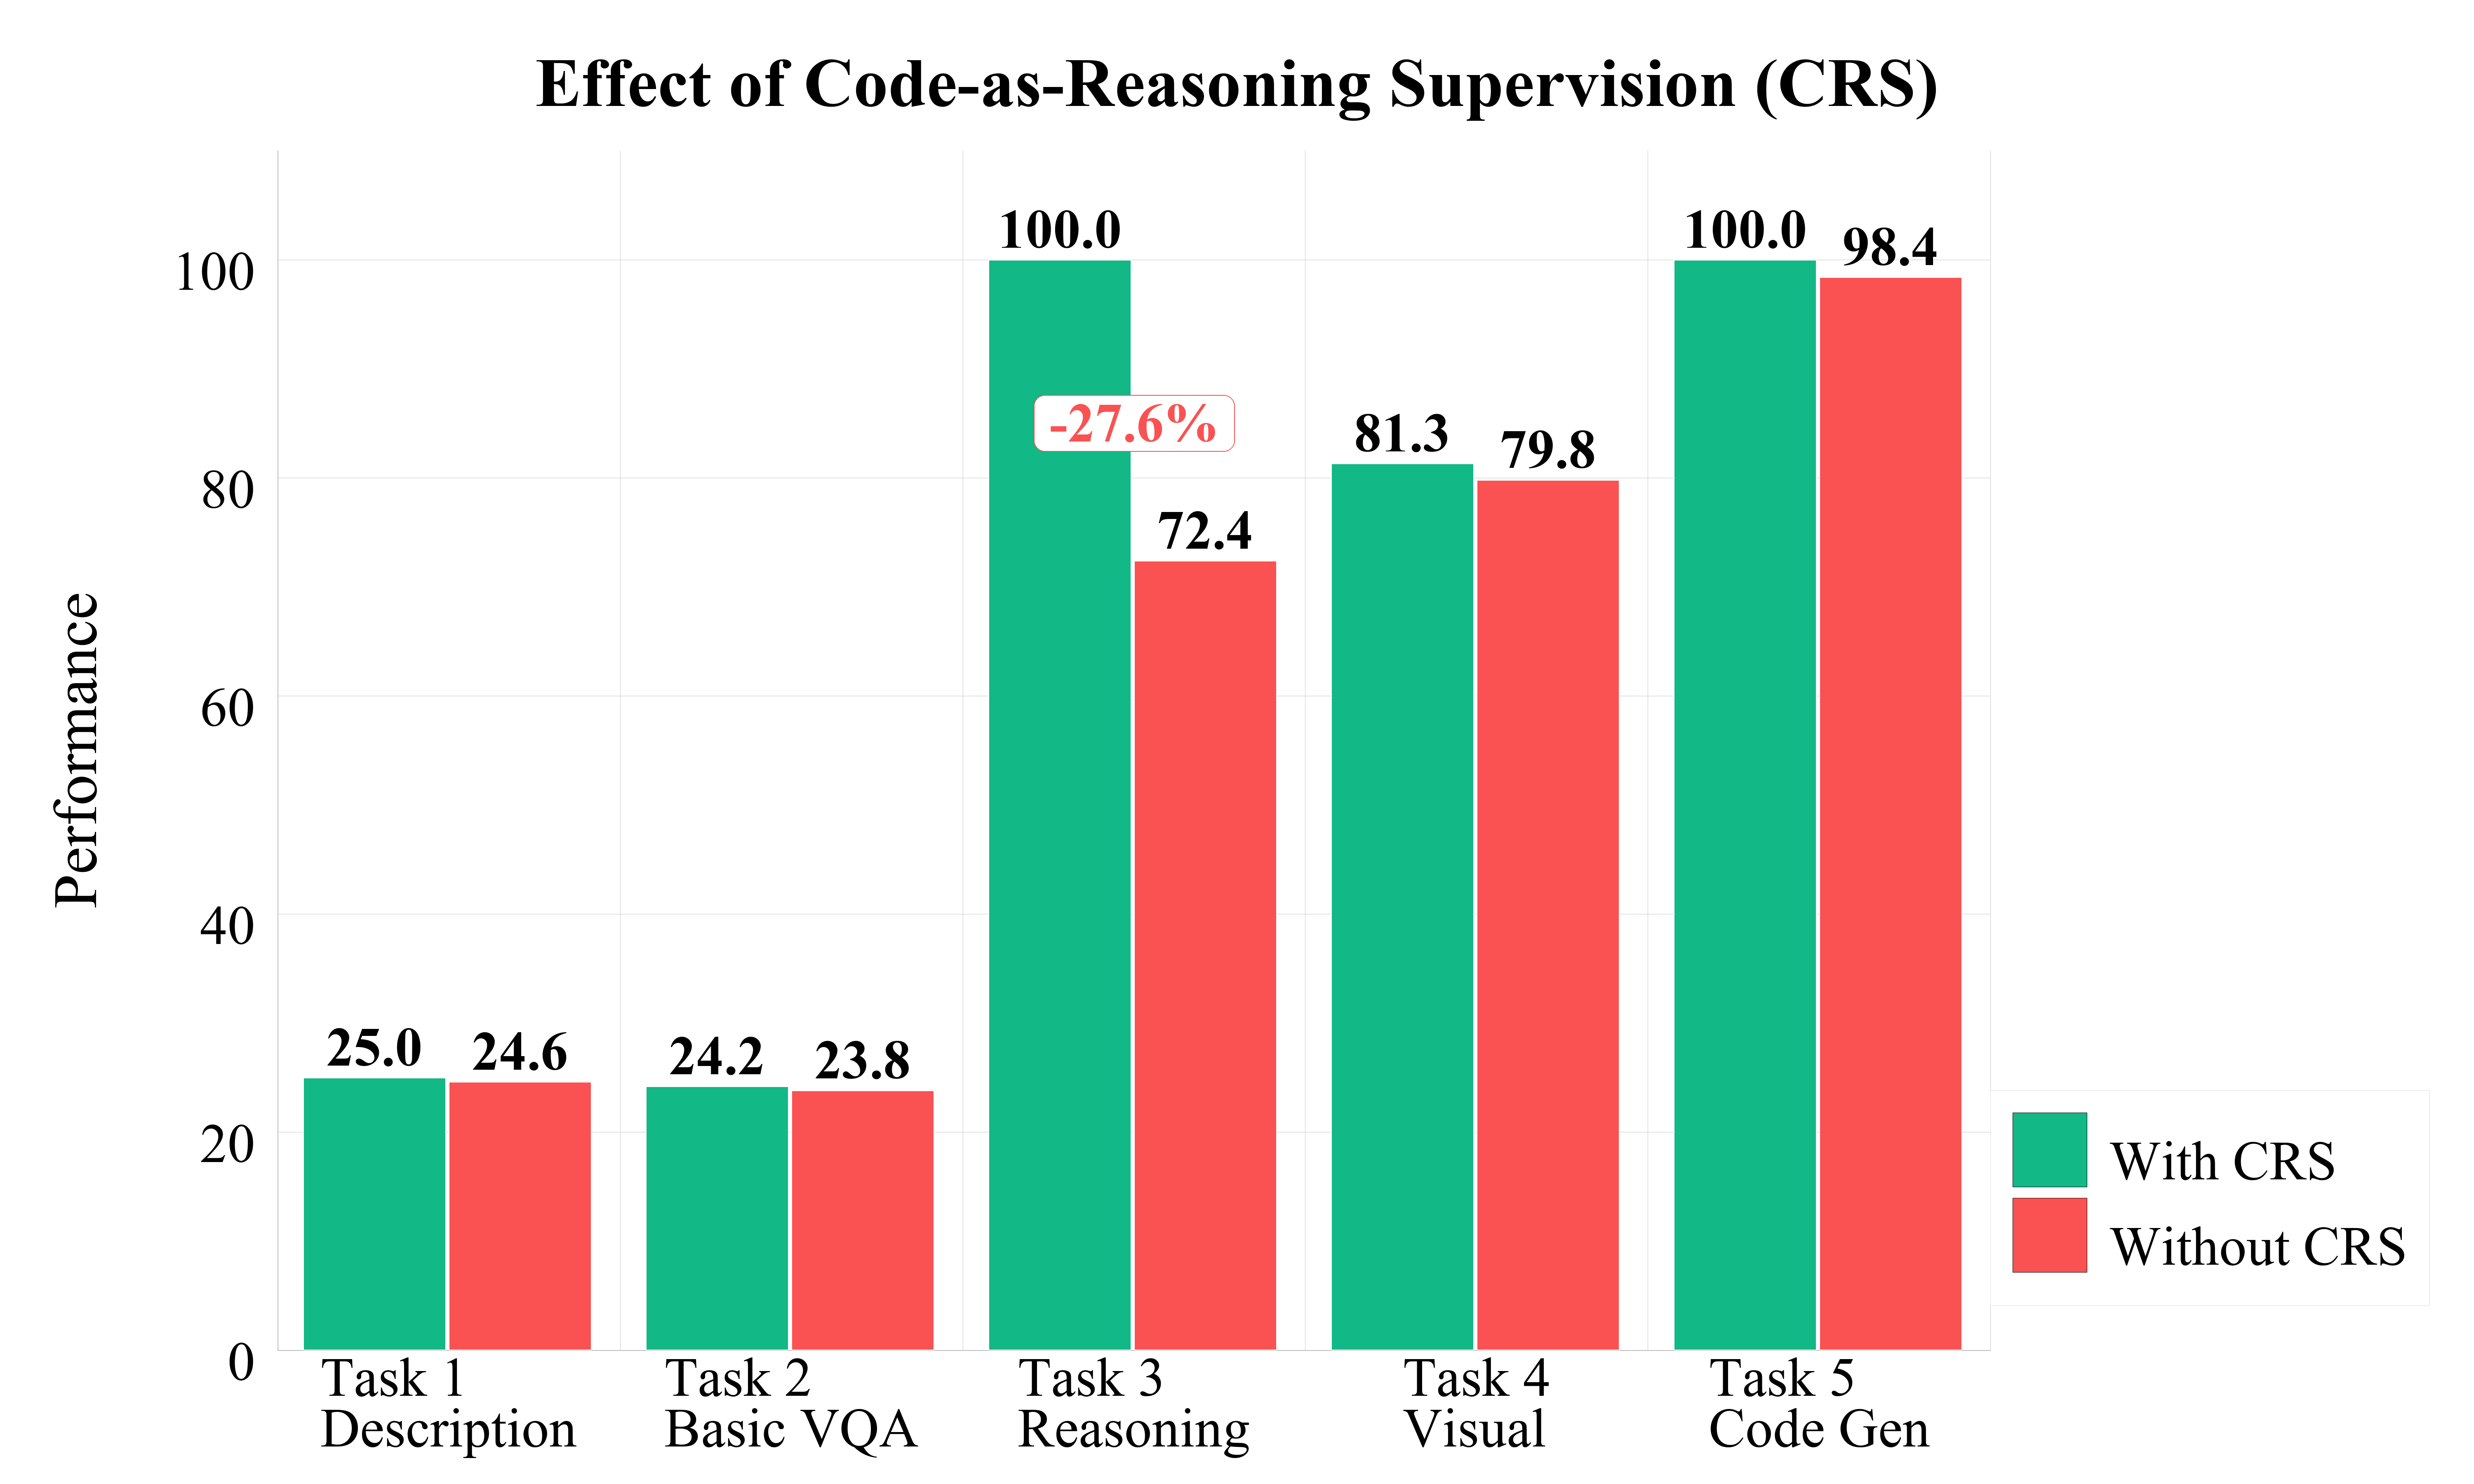
\includegraphics[width=\columnwidth]{figs/fig10_crs_effect.png}
    \caption{Effect of \crs{} on reasoning-intensive tasks. Removing code-based supervision mainly hurts the reasoning stage, confirming that \crs{} targets a specific capability gap rather than acting as a generic training bonus.}
    \label{fig:crs_effect}
\end{figure}

Fig.~\ref{fig:crs_effect} isolates the effect of \crs{}.
The largest drop appears on reasoning-heavy questions, where performance falls from 98.6\% to 74.3\% on the internal reasoning benchmark when \crs{} is removed.
This asymmetry is important: \crs{} is not merely increasing output length or verbosity, but is teaching a distinct computational behavior that later transfers to the routed QA system.

\subsection{Why Adapter Inheritance Matters}
The ablation study identifies adapter inheritance as the largest single contributor, and the reason is structural rather than incidental.
Without inheritance, each stage becomes an isolated fine-tuning run starting from the same pretrained backbone.
The nominal curriculum ordering remains, but knowledge acquired in early stages is no longer available as an initialization for later ones.

The transition from Stage 1 to Stage 3 makes this especially clear.
Stage 1 teaches the model to attend to chart layout, legends, and axis semantics through description.
Stage 2 turns that attention into direct value extraction for short-answer QA.
Stage 3 can then concentrate on multi-step reasoning because the visual grounding and value-reading behaviors have already been partially internalized.
If Stage 3 is trained from the base model instead, it must relearn both grounding and reasoning from only 1,775 reasoning-focused samples, which is exactly the failure mode reflected by the 5.28-point drop in Table~\ref{tab:ablation}.

This observation also clarifies why inheritance matters more than difficulty ordering alone.
Difficulty sorting improves optimization within a stage, but inheritance determines whether the curriculum is truly cumulative across stages.
An ordered task sequence without parameter carryover is not a progressive learner; it is just a collection of separate specialists trained in a prescribed order.

\subsection{Qualitative Examples}
The quantitative results are easier to interpret when viewed through representative behaviors learned by different curriculum components.

\paragraph{How \crs{} structures reasoning.}
A typical Stage-3 supervision target for a question such as ``What percentage of the total does Bus represent?'' first extracts the Bus value, then sums all category values, and finally computes the ratio and converts it to a percentage.
This decomposition is important because it forces the model to expose the intermediate quantities on which the final answer depends.
At benchmark inference time, the routed system still returns direct textual answers, but the reasoning stage has already taught later experts a more explicit computational template than answer-only supervision would provide.

\paragraph{Format learning from early QA stages.}
Another recurring pattern is that the frozen base model often identifies the right values yet responds in a verbose style that is poorly matched to exact-match evaluation.
Stage 2 reduces this mismatch by training concise factual responses as a first-class behavior.
This helps explain why Stage 2 remains such a strong default expert in the routing analysis: many benchmark failures are not failures of perception alone, but failures to present an otherwise plausible answer in the required format.

\paragraph{Persistent perceptual failures.}
The remaining hard cases are less about answer style and more about visual grounding.
Dense bar clusters, small legends, and ambiguous axis bindings still trigger shared failures for both the best fixed expert and the routed system.
This qualitative pattern matches the quantitative error taxonomy in Table~\ref{tab:error}: the main unresolved issues are arithmetic and value extraction, not the absence of a reasoning scaffold.

\subsection{Difficulty Reliability}

To validate \dacds{}, we analyze the difficulty scores assigned to the 1,973 synthetic training samples.
Rather than measuring inter-annotator agreement, we verify that the assigned difficulty levels capture meaningful differences in mathematical complexity.
Table~\ref{tab:difficulty_patterns} groups samples by their question type and reports the mean LLM-assigned difficulty level.
Min/max lookup questions receive the lowest scores (mean 1.0--1.5), while computing variance, which requires multiple statistical operations, receives the highest (mean 5.0).
Intermediate operations---addition, filtering, averaging---fall at the expected intermediate levels.
This monotonic relationship between operation complexity and difficulty score confirms that \dacds{} produces a substantively meaningful ranking, not arbitrary noise.

\begin{table}[!t]
\centering
\footnotesize
\resizebox{\columnwidth}{!}{%
\begin{tabular}{lcc}
\toprule
\textbf{Question Type} & \textbf{Mean Diff.} & \textbf{\# Samples} \\
\midrule
Min/Max lookup      & 1.0--1.5 & 299 \\
Difference          & 2.0      & 98  \\
Percentage          & 2.6      & 196 \\
Sum                 & 2.9      & 493 \\
Count/Filter        & 3.6      & 99  \\
Average/Mean        & 3.7      & 297 \\
Variance            & 5.0      & 100 \\
\midrule
\multicolumn{3}{l}{\textit{Overall 1,973 samples across 5 levels; distribution: 10.4\%/33.5\%/31.8\%/14.2\%/10.1\%.}} \\
\bottomrule
\end{tabular}}
\vspace{4pt}
\caption{Validation of \dacds{} difficulty scores by question type. The assigned levels align monotonically with the mathematical complexity of the operations required to answer each question.}
\label{tab:difficulty_patterns}
\end{table}

Beyond the scoring validity, removing difficulty ordering reduces ChartQA accuracy from 82.12\% to 80.84\% (ablation Table~\ref{tab:ablation}), confirming that easy-to-hard progression contributes a reliable benefit.

\section{Conclusion}
We introduced \fullmethod{} for chart understanding, a framework that structures learning along task complexity and sample difficulty.
The method is supported by \crs{} for explicit executable reasoning supervision and \dacds{} for difficulty-aware sample ordering.
To make the resulting stage experts practical at deployment time, we further proposed \sar{}, a lightweight routing module that selects the most suitable expert for each query.

On ChartQA, \method{}+\sar{} reaches 82.60\% with only 12K synthetic samples, improving over standard LoRA fine-tuning by 6.59 points and over the best fixed single-stage adapter by 0.48 points.
Oracle routing at 87.48\% further shows that the multi-stage experts are complementary, while the current gap to oracle highlights routing as the main target for future improvement.
Across PlotQA and FigureQA, zero-shot transfer results confirm that the learned capabilities generalize beyond the training distribution.

Ablation studies isolate the contribution of each component, with adapter inheritance and task staging providing the largest gains.
The division of labor across components---staging and inheritance building capability progressively, \crs{} strengthening explicit computation, \dacds{} smoothing within-stage optimization, and \sar{} translating specialization into practical inference---helps explain why the complete framework consistently outperforms both standard SFT and one-dimensional curricula.
Meanwhile, error analysis reveals that arithmetic and value-extraction errors remain the dominant failure modes, suggesting that future work should combine curriculum learning with stronger chart-aware numerical grounding.

These results suggest that for multimodal reasoning tasks such as chart understanding, organizing \emph{how} the model learns can be as important as scaling \emph{what} it learns from.

\section*{Limitations}
Our study has several limitations. First, the curriculum is trained primarily on synthetic charts; real-world charts with unusual layouts may induce distribution shift. Second, \sar{} relies on oracle routing labels derived from held-out data; joint end-to-end learning of experts and routing could improve performance further. Third, we focus on five common chart types; broader visualization forms remain out of scope. Fourth, all experiments are in English; multilingual chart understanding remains open.

\appendices
\section{Training Details}
\paragraph{Dataset Composition.}
Fig.~\ref{fig:dataset_dist} visualizes the composition of our synthetic training data.
The chart-type distribution is approximately balanced, with bar and line charts slightly more frequent than area charts.
Difficulty levels are skewed toward easier examples by design, reflecting the curriculum philosophy.

\begin{figure}[!t]
    \centering
    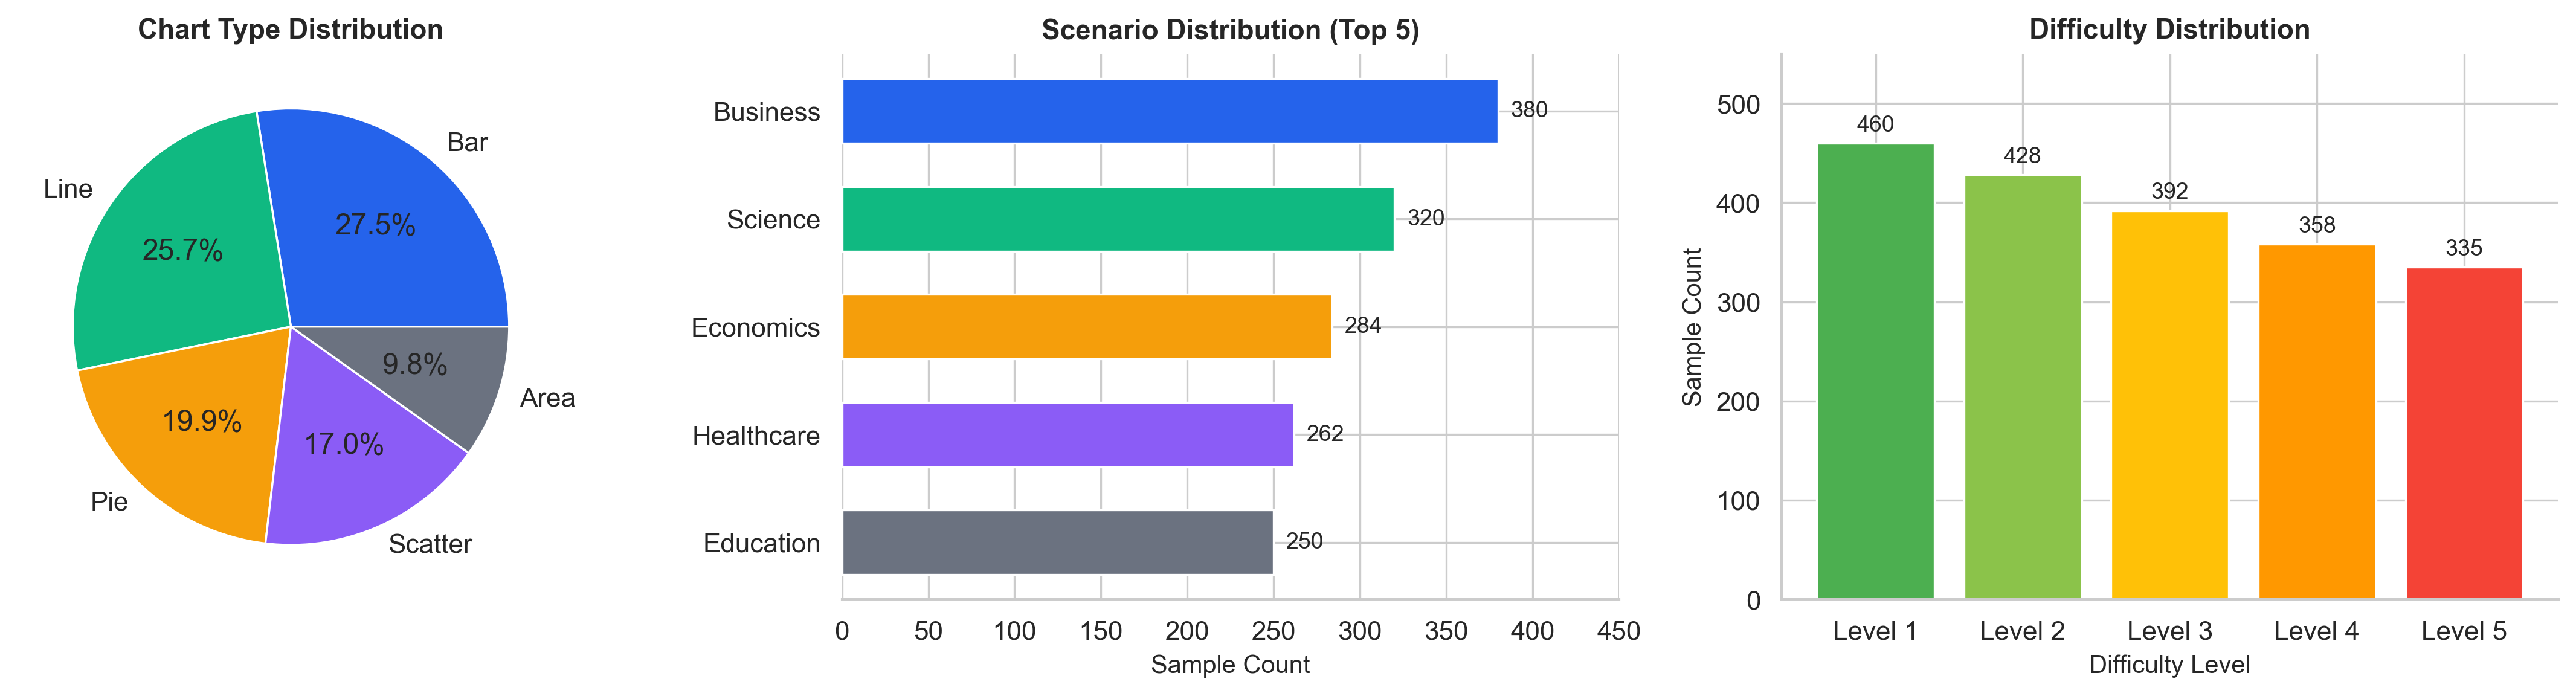
\includegraphics[width=\columnwidth]{figs/fig11_dataset_distribution.png}
    \caption{Distribution of synthetic training data. (a) Chart types. (b) Scenario categories. (c) Difficulty levels.}
    \label{fig:dataset_dist}
\end{figure}

\paragraph{Hyperparameters.}
Table~\ref{tab:hyperparams} lists the stage-wise hyperparameters.
Stage 5 uses a longer maximum sequence length to accommodate code outputs.

\begin{table}[!t]
\centering
\small
\begin{tabular}{lccccc}
\toprule
& \textbf{S1} & \textbf{S2} & \textbf{S3} & \textbf{S4} & \textbf{S5} \\
\midrule
Learning Rate & 1e-4 & 5e-5 & 3e-5 & 3e-5 & 2e-5 \\
Epochs & 10 & 10 & 10 & 10 & 10 \\
Batch Size & 16 & 16 & 16 & 16 & 16 \\
Max Length & 2048 & 2048 & 2048 & 2048 & 4096 \\
LoRA Rank & 8 & 8 & 8 & 8 & 8 \\
LoRA Alpha & 16 & 16 & 16 & 16 & 16 \\
LoRA Dropout & 0.1 & 0.1 & 0.1 & 0.1 & 0.1 \\
\bottomrule
\end{tabular}
\vspace{4pt}
\caption{Hyperparameters for curriculum training.}
\label{tab:hyperparams}
\end{table}

\paragraph{Training Dynamics.}
Table~\ref{tab:training_dynamics} summarizes optimization across stages.
Most stages reach 90\% of final performance within the first two or three epochs, suggesting that inheritance provides a favorable initialization.

\begin{table}[!t]
\centering
\small
\begin{tabular}{lccccc}
\toprule
& \textbf{S1} & \textbf{S2} & \textbf{S3} & \textbf{S4} & \textbf{S5} \\
\midrule
\# Samples & 1,775 & 1,775 & 1,775 & 5,327 & 1,775 \\
Initial Loss & 2.34 & 1.18 & 0.86 & 0.58 & 0.42 \\
Final Loss & 0.667 & 0.381 & 0.268 & 0.173 & 0.109 \\
Reduction (\%) & 71.5 & 67.7 & 68.8 & 70.2 & 74.0 \\
Epochs to 90\% & 3 & 2 & 2 & 4 & 2 \\
Wall-clock (h) & 3.6 & 2.7 & 2.5 & 9.6 & 2.5 \\
\bottomrule
\end{tabular}
\vspace{4pt}
\caption{Training dynamics across stages. Stage 4 is the most time-consuming because it contains roughly three times as many samples as the other stages.}
\label{tab:training_dynamics}
\end{table}

\section{Additional Results}
\paragraph{Multi-Task Profile.}
Table~\ref{tab:task_profile} compares curriculum training against standard SFT on the five internal task families.
The largest gains occur on reasoning and code-related tasks, which aligns with the design motivation of \crs{} and staged capability building.

\begin{table}[!t]
\centering
\small
\begin{tabular}{lcc}
\toprule
\textbf{Task Type} & \textbf{\method{}} & \textbf{Standard SFT} \\
\midrule
T1: Description (BLEU) & 25.0 & 12.8 \\
T2: Basic VQA (Acc.) & 25.1 & 18.4 \\
T3: Reasoning (Acc.) & 98.6 & 60.2 \\
T4: Visual Analysis (Acc.) & 82.1 & 55.4 \\
T5: Code Generation (Acc.) & 99.2 & 63.1 \\
\bottomrule
\end{tabular}
\vspace{4pt}
\caption{Performance across internal task families. Curriculum learning most strongly improves reasoning-heavy capabilities.}
\label{tab:task_profile}
\end{table}

\bibliographystyle{IEEEtran}
\bibliography{references}

\end{document}

